\documentclass[12pt,a4paper,UTF8]{ctexart}
\usepackage{geometry}
	\geometry{left=2.5cm,right=2.5cm,top=2cm,bottom=2cm}
\usepackage{xeCJK,amsmath,paralist,enumitem,booktabs,multirow,graphicx,subfig,setspace}
	\setlength{\parindent}{2em}
\usepackage[colorlinks,linkcolor=blue,urlcolor=blue]{hyperref}

%%%%%%%%%%%%%%%%%%%%%%%%%正文开始%%%%%%%%%%%%%%%%%%%%%%%%%%
\begin{document}

\title{\vspace{-2cm}\LARGE\bfseries B10/B16 夫琅禾费单缝衍射实验与仿真\footnotemark[1]}
\author{\large\textit{黄子维}$^{1}$\footnotemark[2],\large\textit{黄睿杰}$^{2}$\footnotemark[3] \\ 
\small{1,2 \textit{中山大学 中山医学院,广东 广州 }510275}}
\date{}
\maketitle
\setcounter{page}{0}
\thispagestyle{empty}
\vspace{-1.5em}
\begin{spacing}{2.0}
{\bfseries 摘 {} 要:}
夫琅禾费单缝衍射是指平行光通过尺寸接近波长的狭缝时,偏离传播方向而在无穷远处形成衍射条纹的现象。
其衍射条纹具有一个能量集中的主极大,其余次极大对称分布,且光强随级次升高而迅速衰减。
在条纹中心附近,次级条纹角宽度近似等于主极大的半角宽。
本实验中,我们使用光功率计测量氦氖激光夫琅禾费单缝衍射各级条纹相对光强分布,并将实验结果和理论曲线进行对比。
同时我们检查了光功率计是否工作在线性区。最后我们使用$Seelight$光学仿真平台进行了仿真实验。

我们首先测量了氦氖激光夫琅禾费单缝衍射各级条纹相对光强分布,与理论曲线对比后发现主极大符合较好,但次级大相对光强偏低,且暗纹处光强并非为零。
同时我们计算了各级暗纹距离,发现与理论预测相符。
接下来,我们使用光功率计测量了不同距离处溴钨灯光的光功率,证实了光功率计工作在线性区内。
最后,我们在$Seelight$光学平台上使用同样的实验参数搭建了实验模型,进行了仿真实验,并验证仿真结果。

\begin{figure}[htbp]
	\centering
	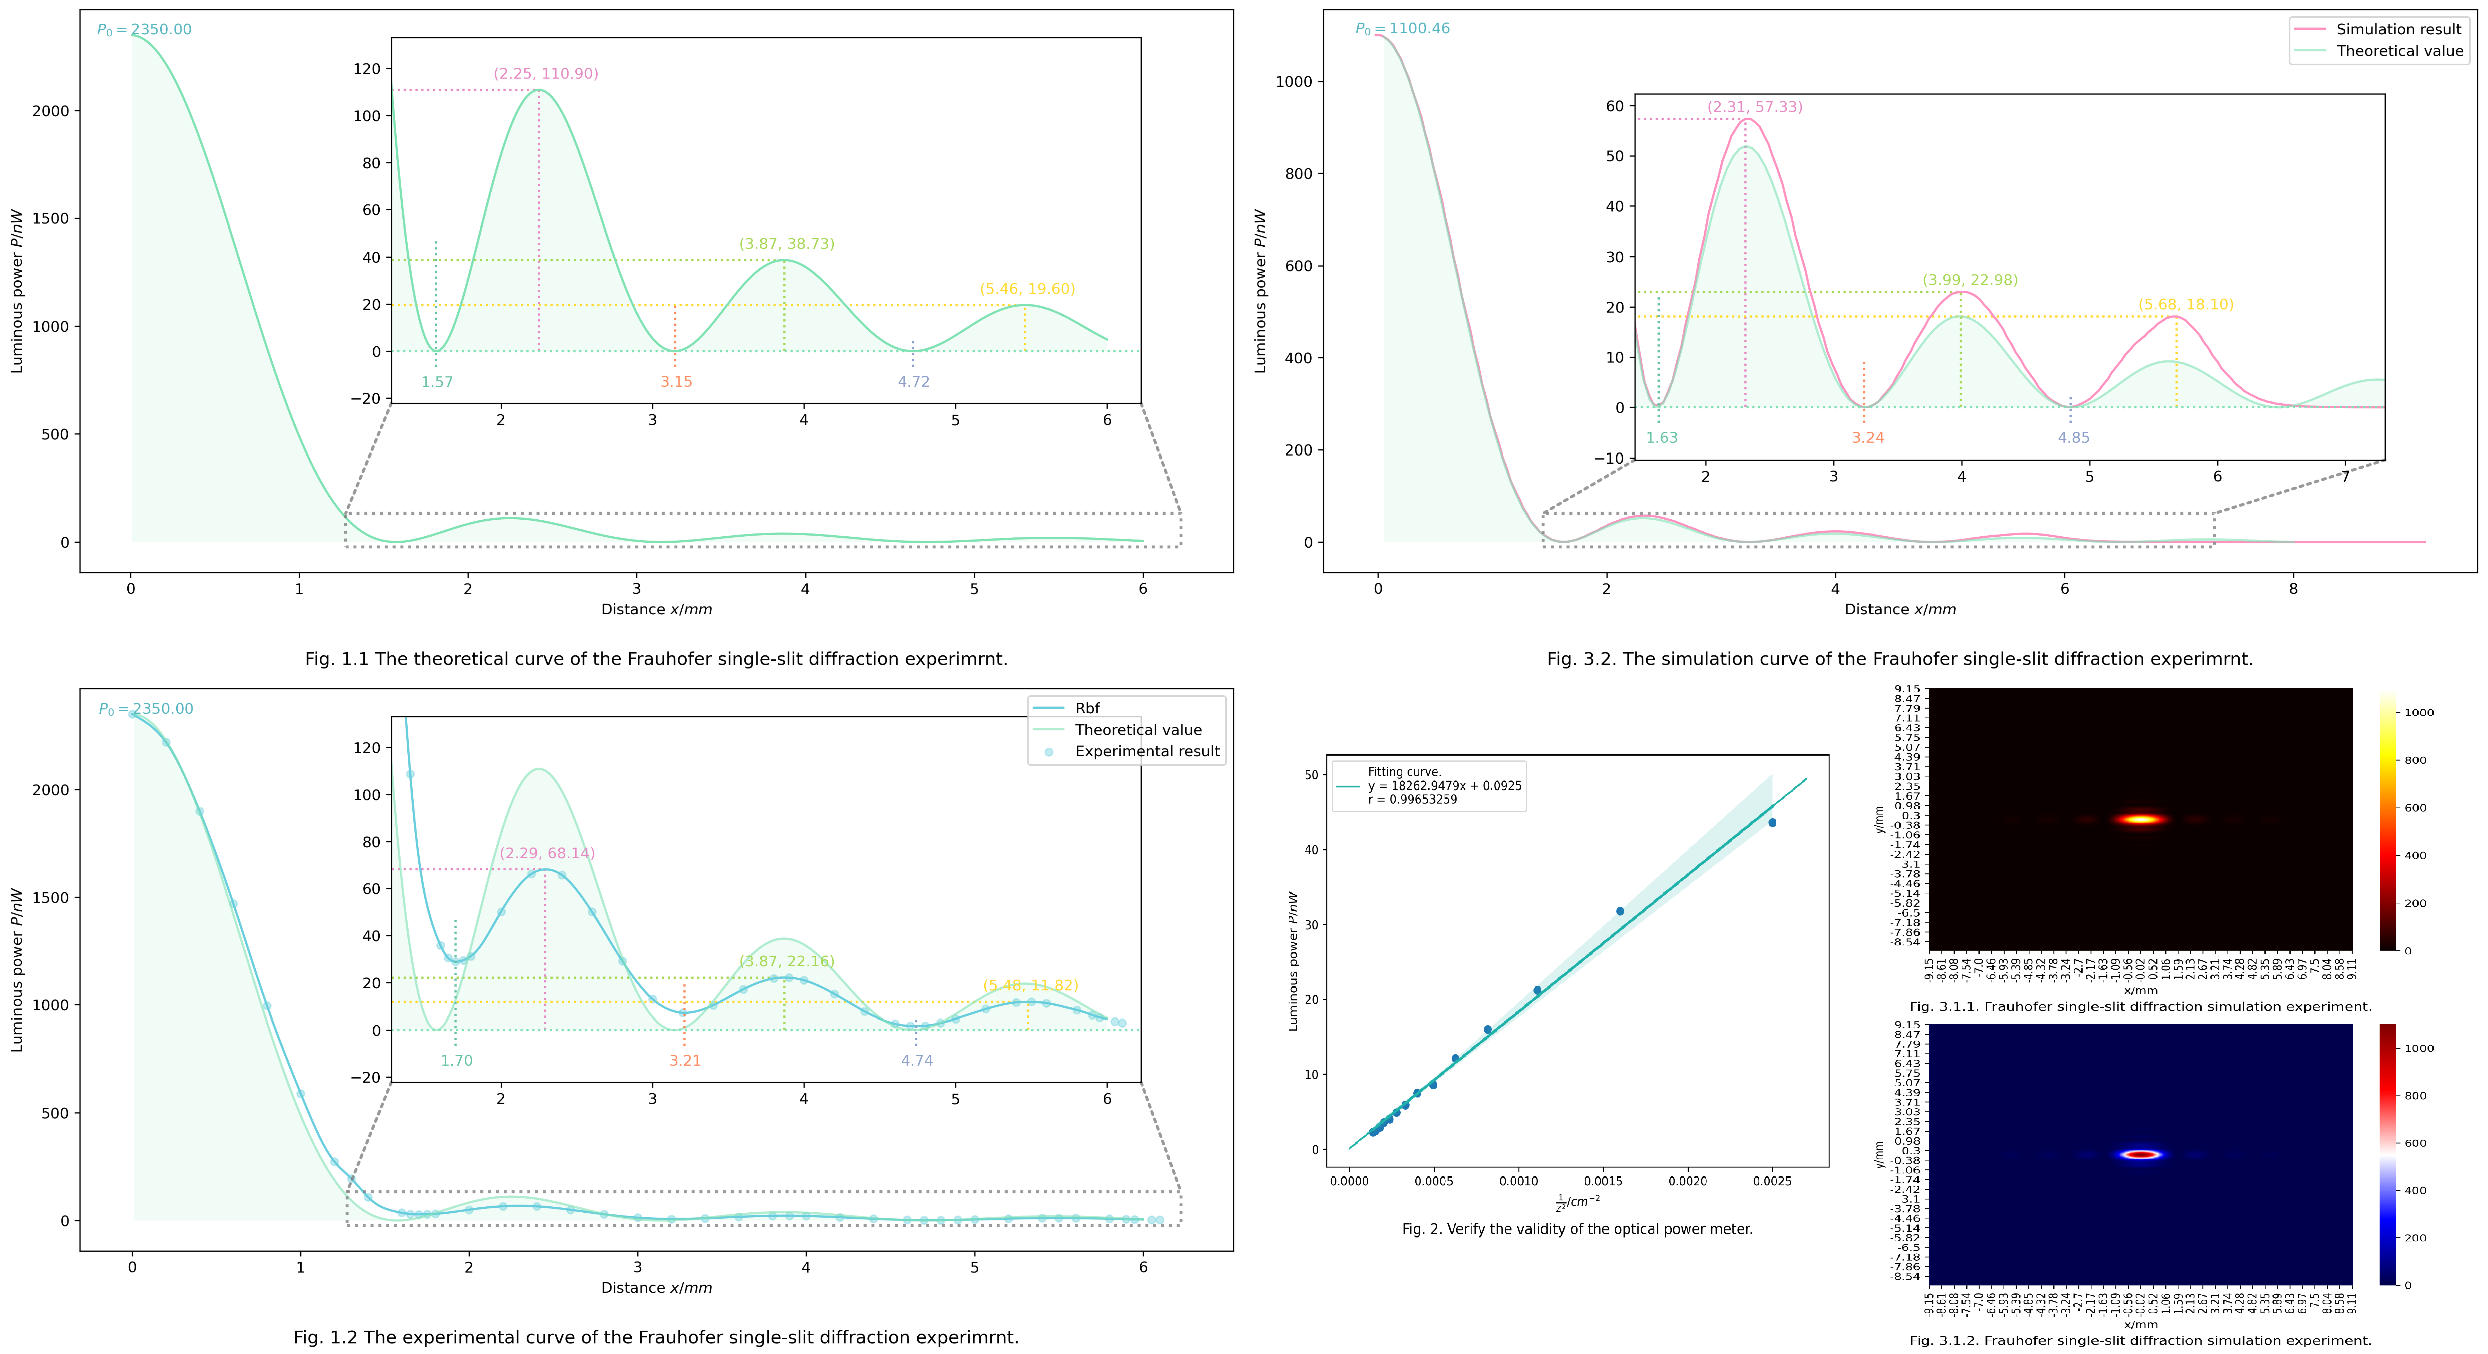
\includegraphics[width=0.7\textwidth]{attachments/Fig.0.pdf}
	\caption{夫琅禾费单缝衍射}
	\label{fig:0}
\end{figure}
\par
\vspace{-0.5em}
\bfseries{关键词}: 氦氖激光夫琅禾费单缝衍射,相对光强分布,光学仿真实验
\vspace{0.5em}
\end{spacing}

\renewcommand{\thefootnote}{\fnsymbol{footnote}}
\footnotetext[1]{由中山大学物理学院陆佑堂提供器材和指导。}
\footnotetext[2]{通信作者,20980066,\url{huangzw29@mail2.sysu.edu.cn}}
\footnotetext[3]{实验参与人,20980062}

%%%%%%%%附录:数据处理%%%%%%%
\newpage
\pagestyle{plain}
\begin{center}
\LARGE\textbf{实验B10/B16 夫琅禾费单缝衍射实验与仿真}
\end{center}

%%信息
\begin{doublespacing}
	\centering
	\begin{tabular}{ll}
	 & \\
	{\CJKfontspec{Droid Sans Fallback} 实验人:黄子维 20980066} & {\CJKfontspec{Droid Sans Fallback}合作者:黄睿杰 20980062}\\
	{\CJKfontspec{Droid Sans Fallback} 实验时间:2021.10.21~星期四~上午} & {\CJKfontspec{Droid Sans Fallback} 室温:25$^{\circ}$C~相对湿度:62\%}
	\end{tabular}
\end{doublespacing}
\subsection*{【实验参数】}

\begin{table}[htbp]
	\centering
	\begin{tabular}{cc}
	\toprule
	参数 &值 \\
	\midrule
	出光口到狭缝距离 d &3cm \\
	狭缝与光功率计间距离 D &87cm  \\
	狭缝宽 a &0.340mm \\
	狭缝长   &2.5cm \\
	He-Ne激光波长	&632.8nm \\
	观察屏尺寸	&$15cm \times 15cm$ \\
	\bottomrule
    \end{tabular}
	\caption{\textbf{实验参数}}
	\label{tab:0}
\end{table}

\subsection*{【数据处理及分析】}
\subsubsection*{1. 夫琅禾费单缝衍射实验}
根据夫琅禾费单缝衍射理论公式,衍射图样中光强分布为:
\begin{equation}\label{eq:1.1}
	I = I_0\frac{sin^2(\frac{\pi asin\theta}{\lambda})}{(\frac{\pi asin\theta}{\lambda})^2}
\end{equation}
小角近似:
\begin{equation}\label{eq:1.2}
	sin\theta \approx tan\theta = \frac{x}{D}
\end{equation}
实验中,光功率计接受面积始终不变,测得的光功率与光强成正比。
\begin{equation}\label{eq:1.3}
	P \propto I
\end{equation}
综合上述,得光功率分布:
\begin{equation}\label{eq:1.4}
	P = P_0\frac{sin^2(\frac{\pi ax}{D \lambda})}{(\frac{\pi ax}{D \lambda})^2}
\end{equation}
相对光强:
\begin{equation}\label{eq:1.5}
	I' = \frac{I}{I_0} = \frac{P}{P_0} = \frac{sin^2(\frac{\pi ax}{D \lambda})}{(\frac{\pi ax}{D \lambda})^2}
\end{equation}
根据上述计算,代入表\ref{tab:0}相关参数,作出夫琅禾费单缝衍射理论曲线,如图\ref{fig:1.1}所示。

实验使用光功率计测量氦氖激光夫琅禾费单缝衍射各级条纹光强分布,如图\ref{fig:1.2}所示。

\begin{figure}[htbp]
	\centering
	\subfloat[理论曲线]{\label{fig:1.1}
	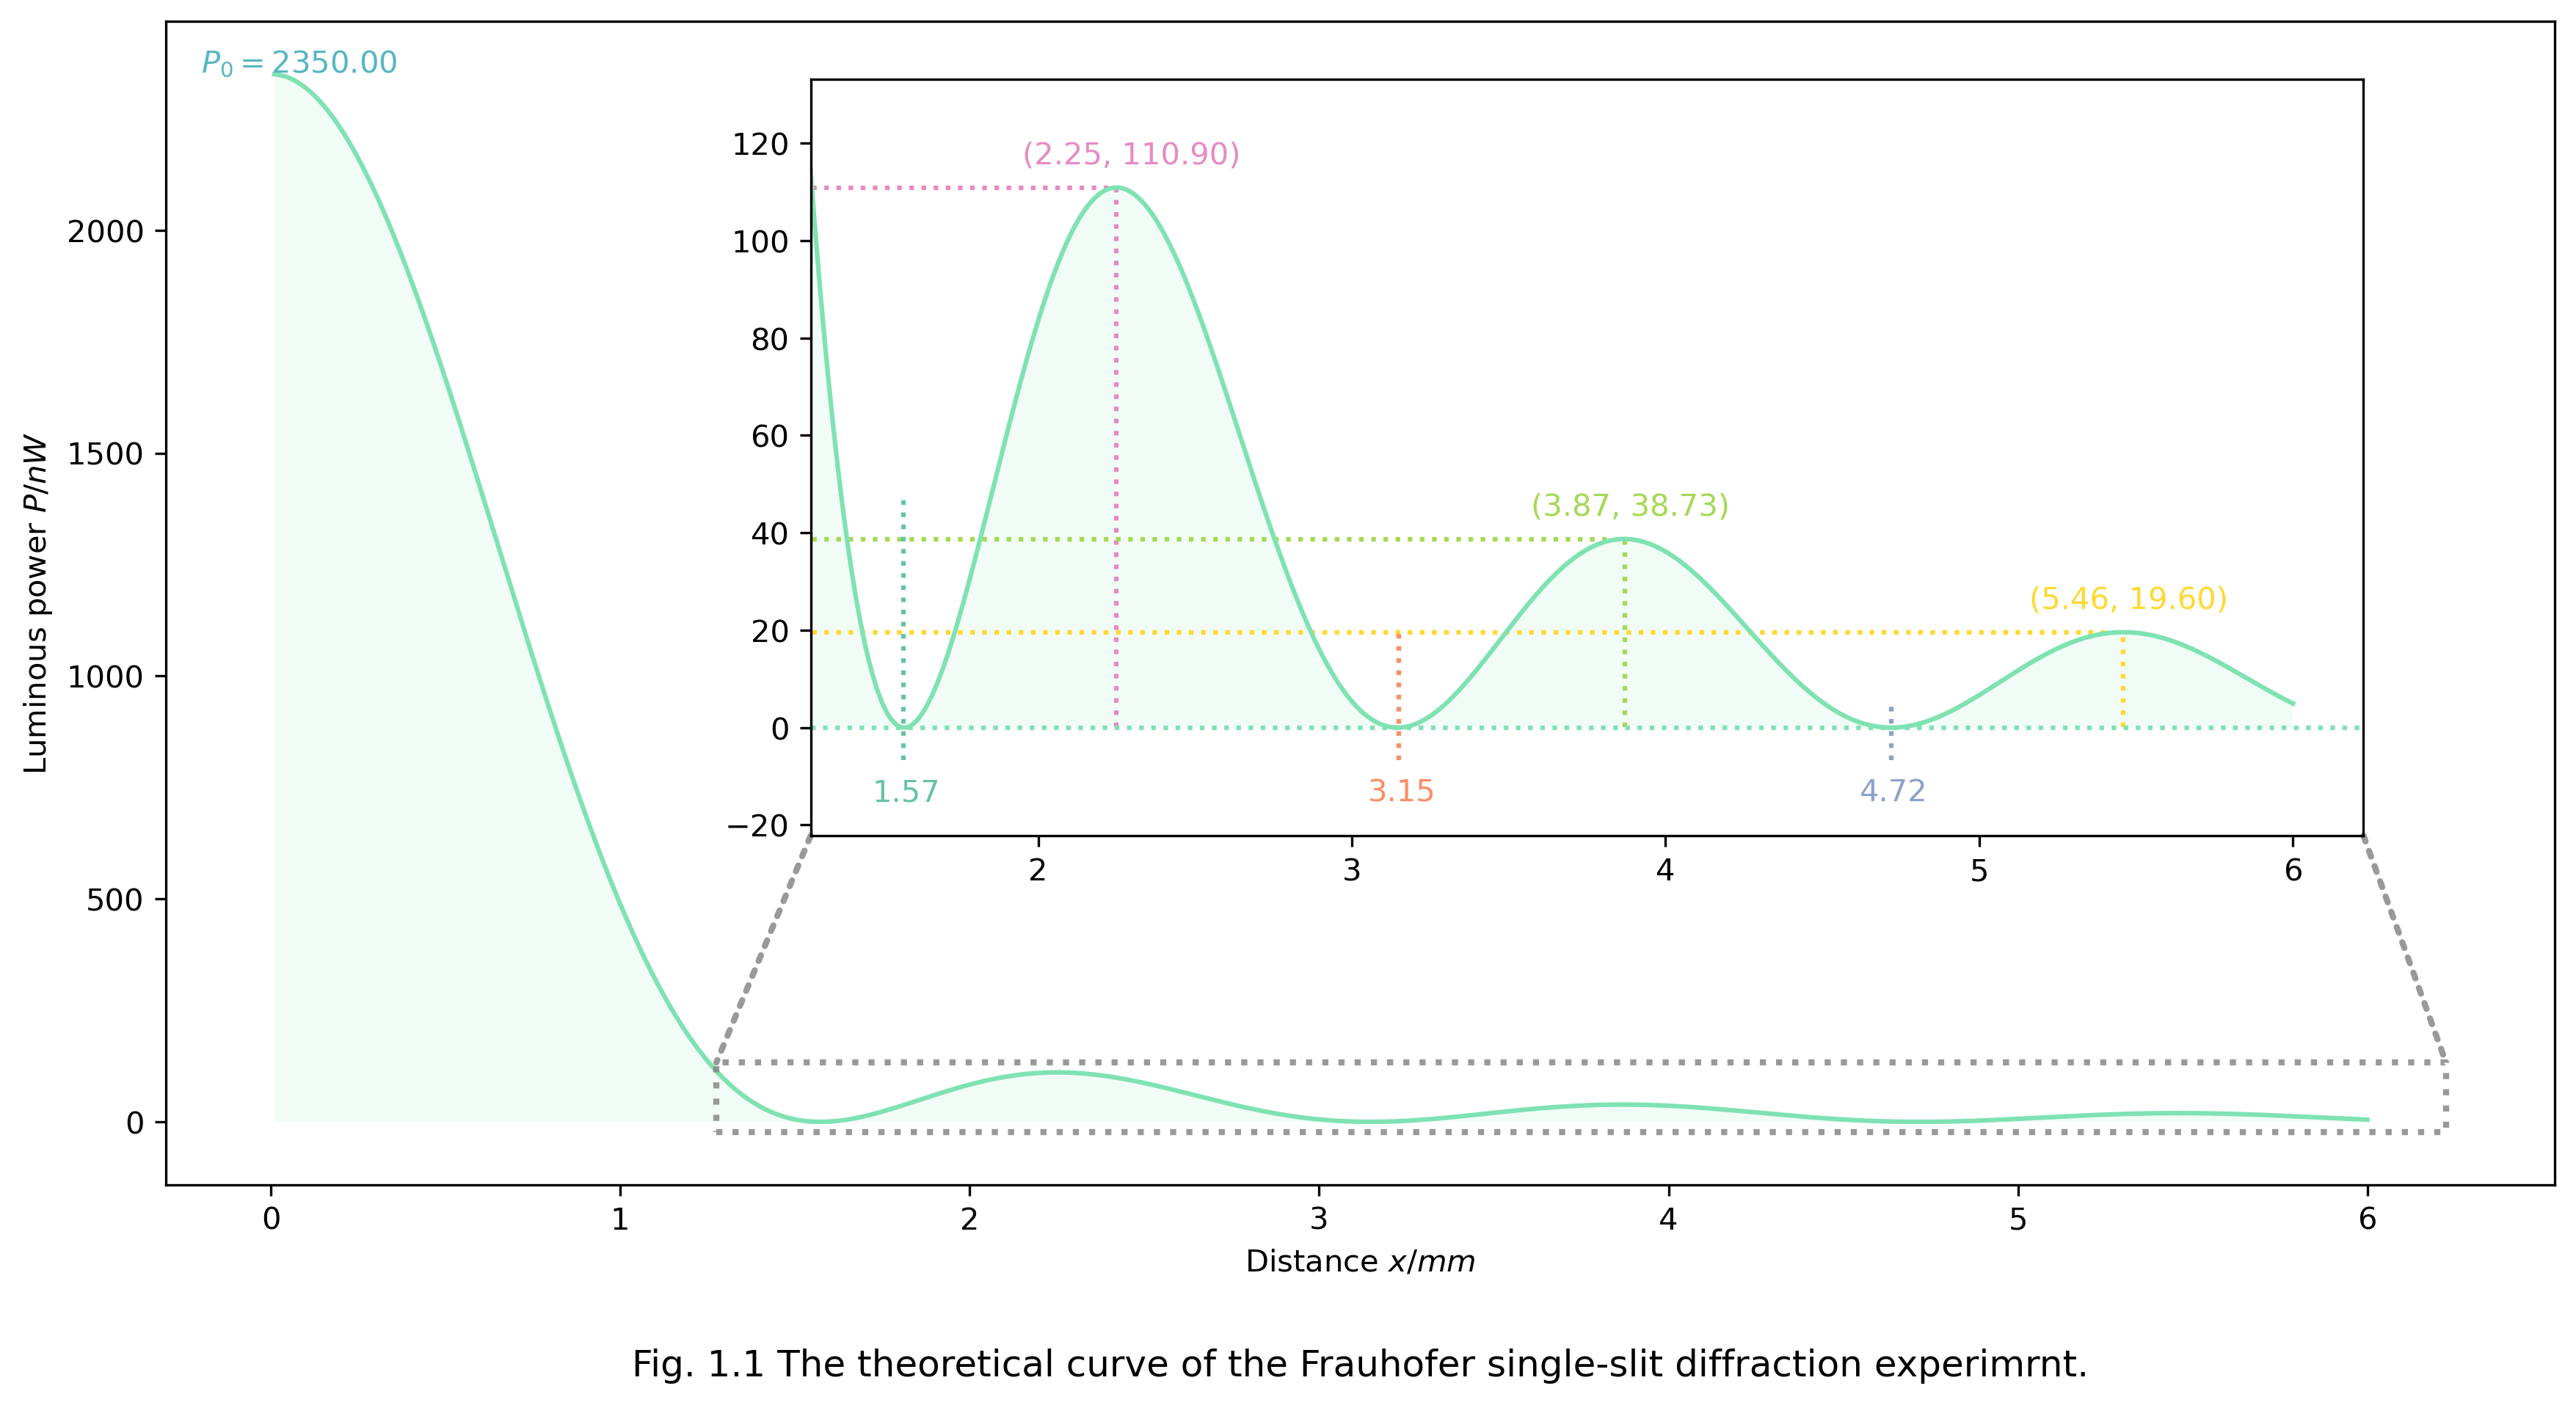
\includegraphics[width=0.6\textwidth]{attachments/Fig.1.1.png}
	}
	
	\subfloat[实验曲线]{\label{fig:1.2}
	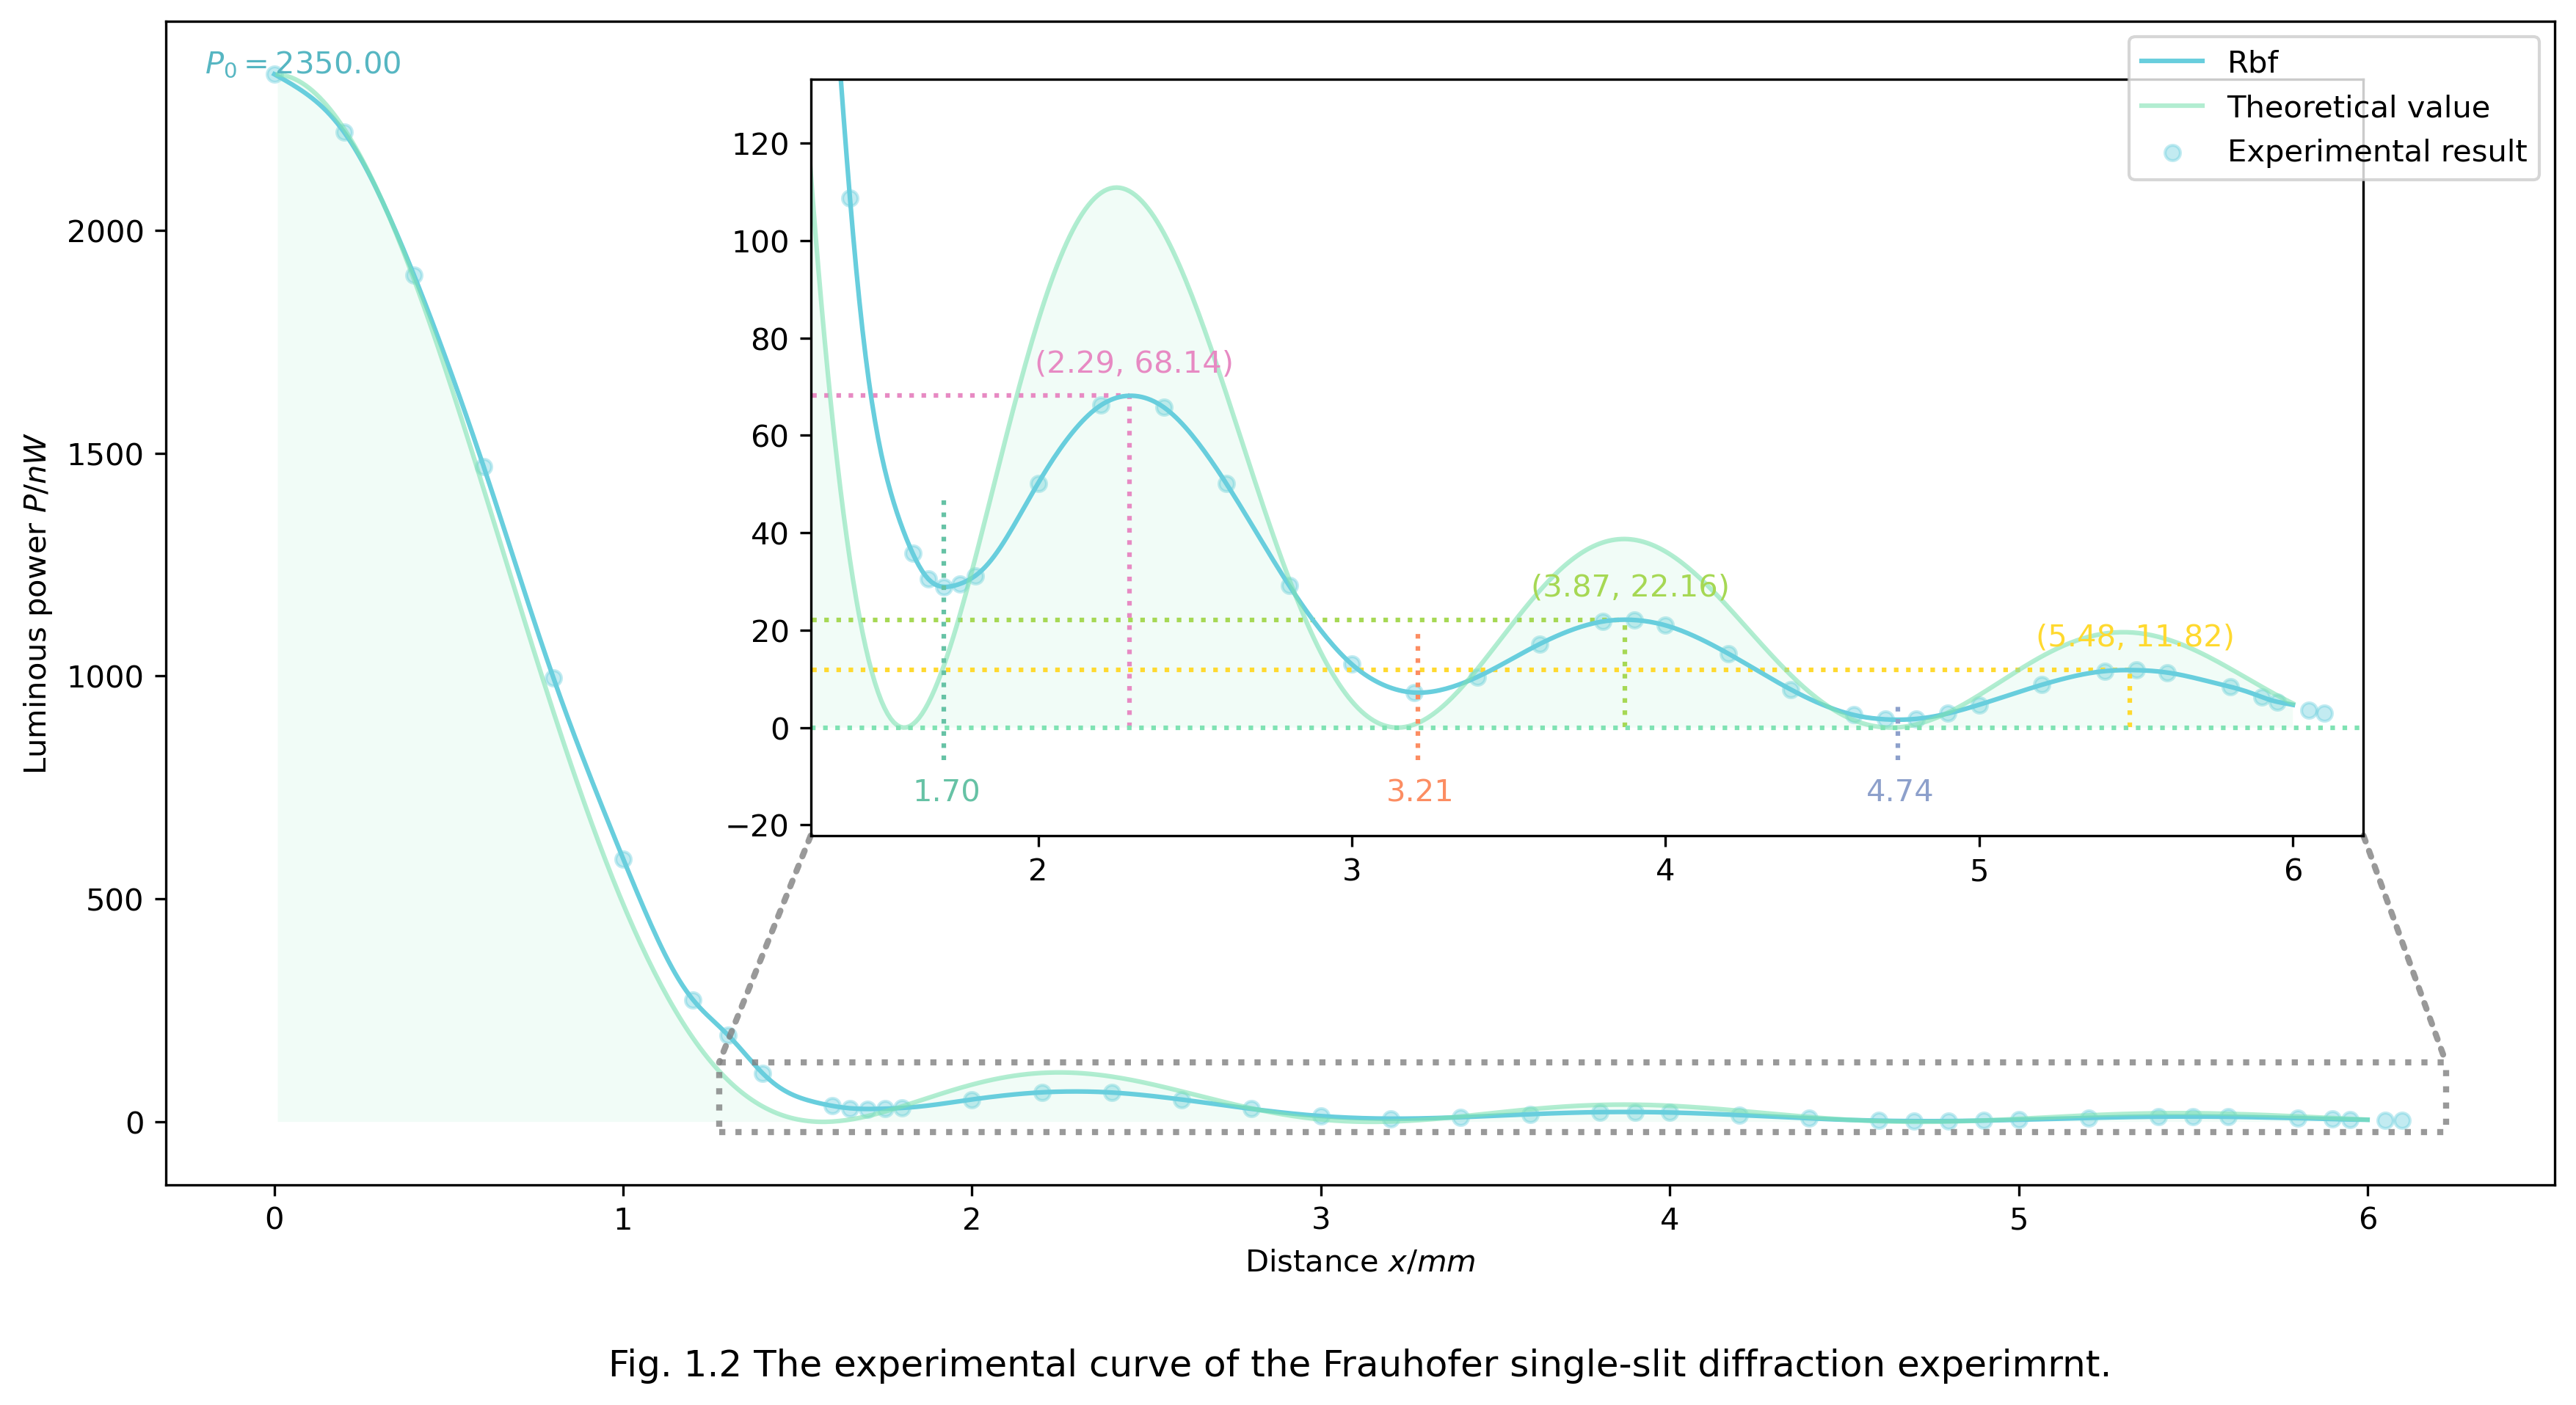
\includegraphics[width=0.6\textwidth]{attachments/Fig.1.2.png}
	}
	\caption{夫琅禾费单缝衍射实验}
\end{figure}
	
我们发现,实验结果中,零级主极大条纹光强分布与理论曲线符合较好,但次级大相对光强偏低。
条纹各次级大峰值与理论对照以及相对误差如表\ref{tab:1.1}。
($P_{the}$:理论光功率;$P_{exp}$:实验光功率;$I'_{the}$:理论相对光强;$I'_{exp}$:实验相对光强)。
此外,我们发现理论预测的暗纹位置光强并非为零。
综合分析,我们认为偏差较大的可能原因为光功率计探头受光面积并非理想近似于零,
测量得到的光功率为探头中心附近一段距离内光功率的平均值,
因此在条纹较为致密的情况下测量效果并不理想,在光功率较低时该效应更加明显。

同时,我们测量了各次极大及各级暗纹的位置,结果如表\ref{tab:1.2}和表\ref{tab:1.3}。
实验值相对误差较小,与理论预测较相符。
计算暗条纹间距为$1.51mm$和$1.53mm$,平均值为$1.52mm$,与理论值$1.62mm$相比相对误差为$6.17\%$

\begin{table}[htbp]
	\centering
	\begin{tabular}{cccccc}
	\toprule
	条纹级次 &$P_{the}/nW$ &$P_{exp}/nW$ &$I'_{the}$ &$I'_{exp}$ &相对误差 \\
	\midrule
	1 &110.890784 &68.143629 &0.047188 &0.028997 &38.55\% \\
	2  &38.727635 &22.162001 &0.016480 &0.009431 &42.77\% \\
	3  &19.599686 &11.817545  &0.008340 &0.005029 &39.71\% \\
	\bottomrule
    \end{tabular}
	\caption{\textbf{次级大条纹峰值}}
	\label{tab:1.1}
\end{table}

\begin{table}[htbp]
	\centering
		\begin{tabular}{cccc}
			\toprule
			条纹级次	&理论位置$/mm$	&实验位置$/mm$	&相对误差 \\
			\midrule
			1  &2.32  &2.29  &1.29\% \\
			2  &3.98  &3.87  &2.76\% \\
			3  &5.62  &5.48  &2.49\% \\	
			\bottomrule
		\end{tabular}
		\caption{\textbf{次级大条纹位置}}
		\label{tab:1.2}
\end{table}

\begin{table}[htbp]
    \centering
		\begin{tabular}{cccc}
			\toprule
			条纹级次	&理论位置$/mm$	&实验位置$/mm$	&相对误差 \\
			\midrule
			1  &1.62  &1.70  &-4.94\% \\
			2  &3.24  &3.21   &0.93\% \\
			3  &4.86  &4.74   &2.47\% \\	
			\bottomrule
		\end{tabular}
		\caption{\textbf{暗纹位置}}
		\label{tab:1.3}
\end{table}

\subsubsection*{2. 验证光功率计是否工作在线性区}
我们在距离溴钨灯不同位置$(Z \in [20cm , 85cm])$使用光功率计测量光功率,实验结果如表\ref{tab:2}。                                         
作拟合直线如图\ref{fig:2},相关系数$r> 0.995$,这就验证了光功率计工作在线性区。

\begin{figure}[htbp]
\begin{minipage}{0.5\textwidth}
	\centering
	\begin{tabular}{ccc}
	\toprule
	距离$Z/cm$ &光功率$P/nW$ &$\frac{1}{Z^2}/cm^{-2}$ \\
	\midrule
	20  &43.6  &0.002500 \\
	25  &31.8  &0.001600 \\
	30  &21.2  &0.001111 \\
	35  &16.0  &0.000816 \\
	40  &12.1  &0.000625 \\
	45  & 8.6  &0.000494 \\
	50  & 7.5  &0.000400 \\
	55  & 5.9  &0.000331 \\
	60  & 4.9  &0.000278 \\
	65  & 4.0  &0.000237 \\
	70  & 3.6  &0.000204 \\
	75  & 2.9  &0.000178 \\
	80  & 2.5  &0.000156 \\
	85  & 2.3  &0.000138 \\
	\bottomrule
    \end{tabular}
	\caption{\textbf{不同距离光功率}}
	\label{tab:2}
\end{minipage}
\begin{minipage}{0.5\textwidth}
    \centering
	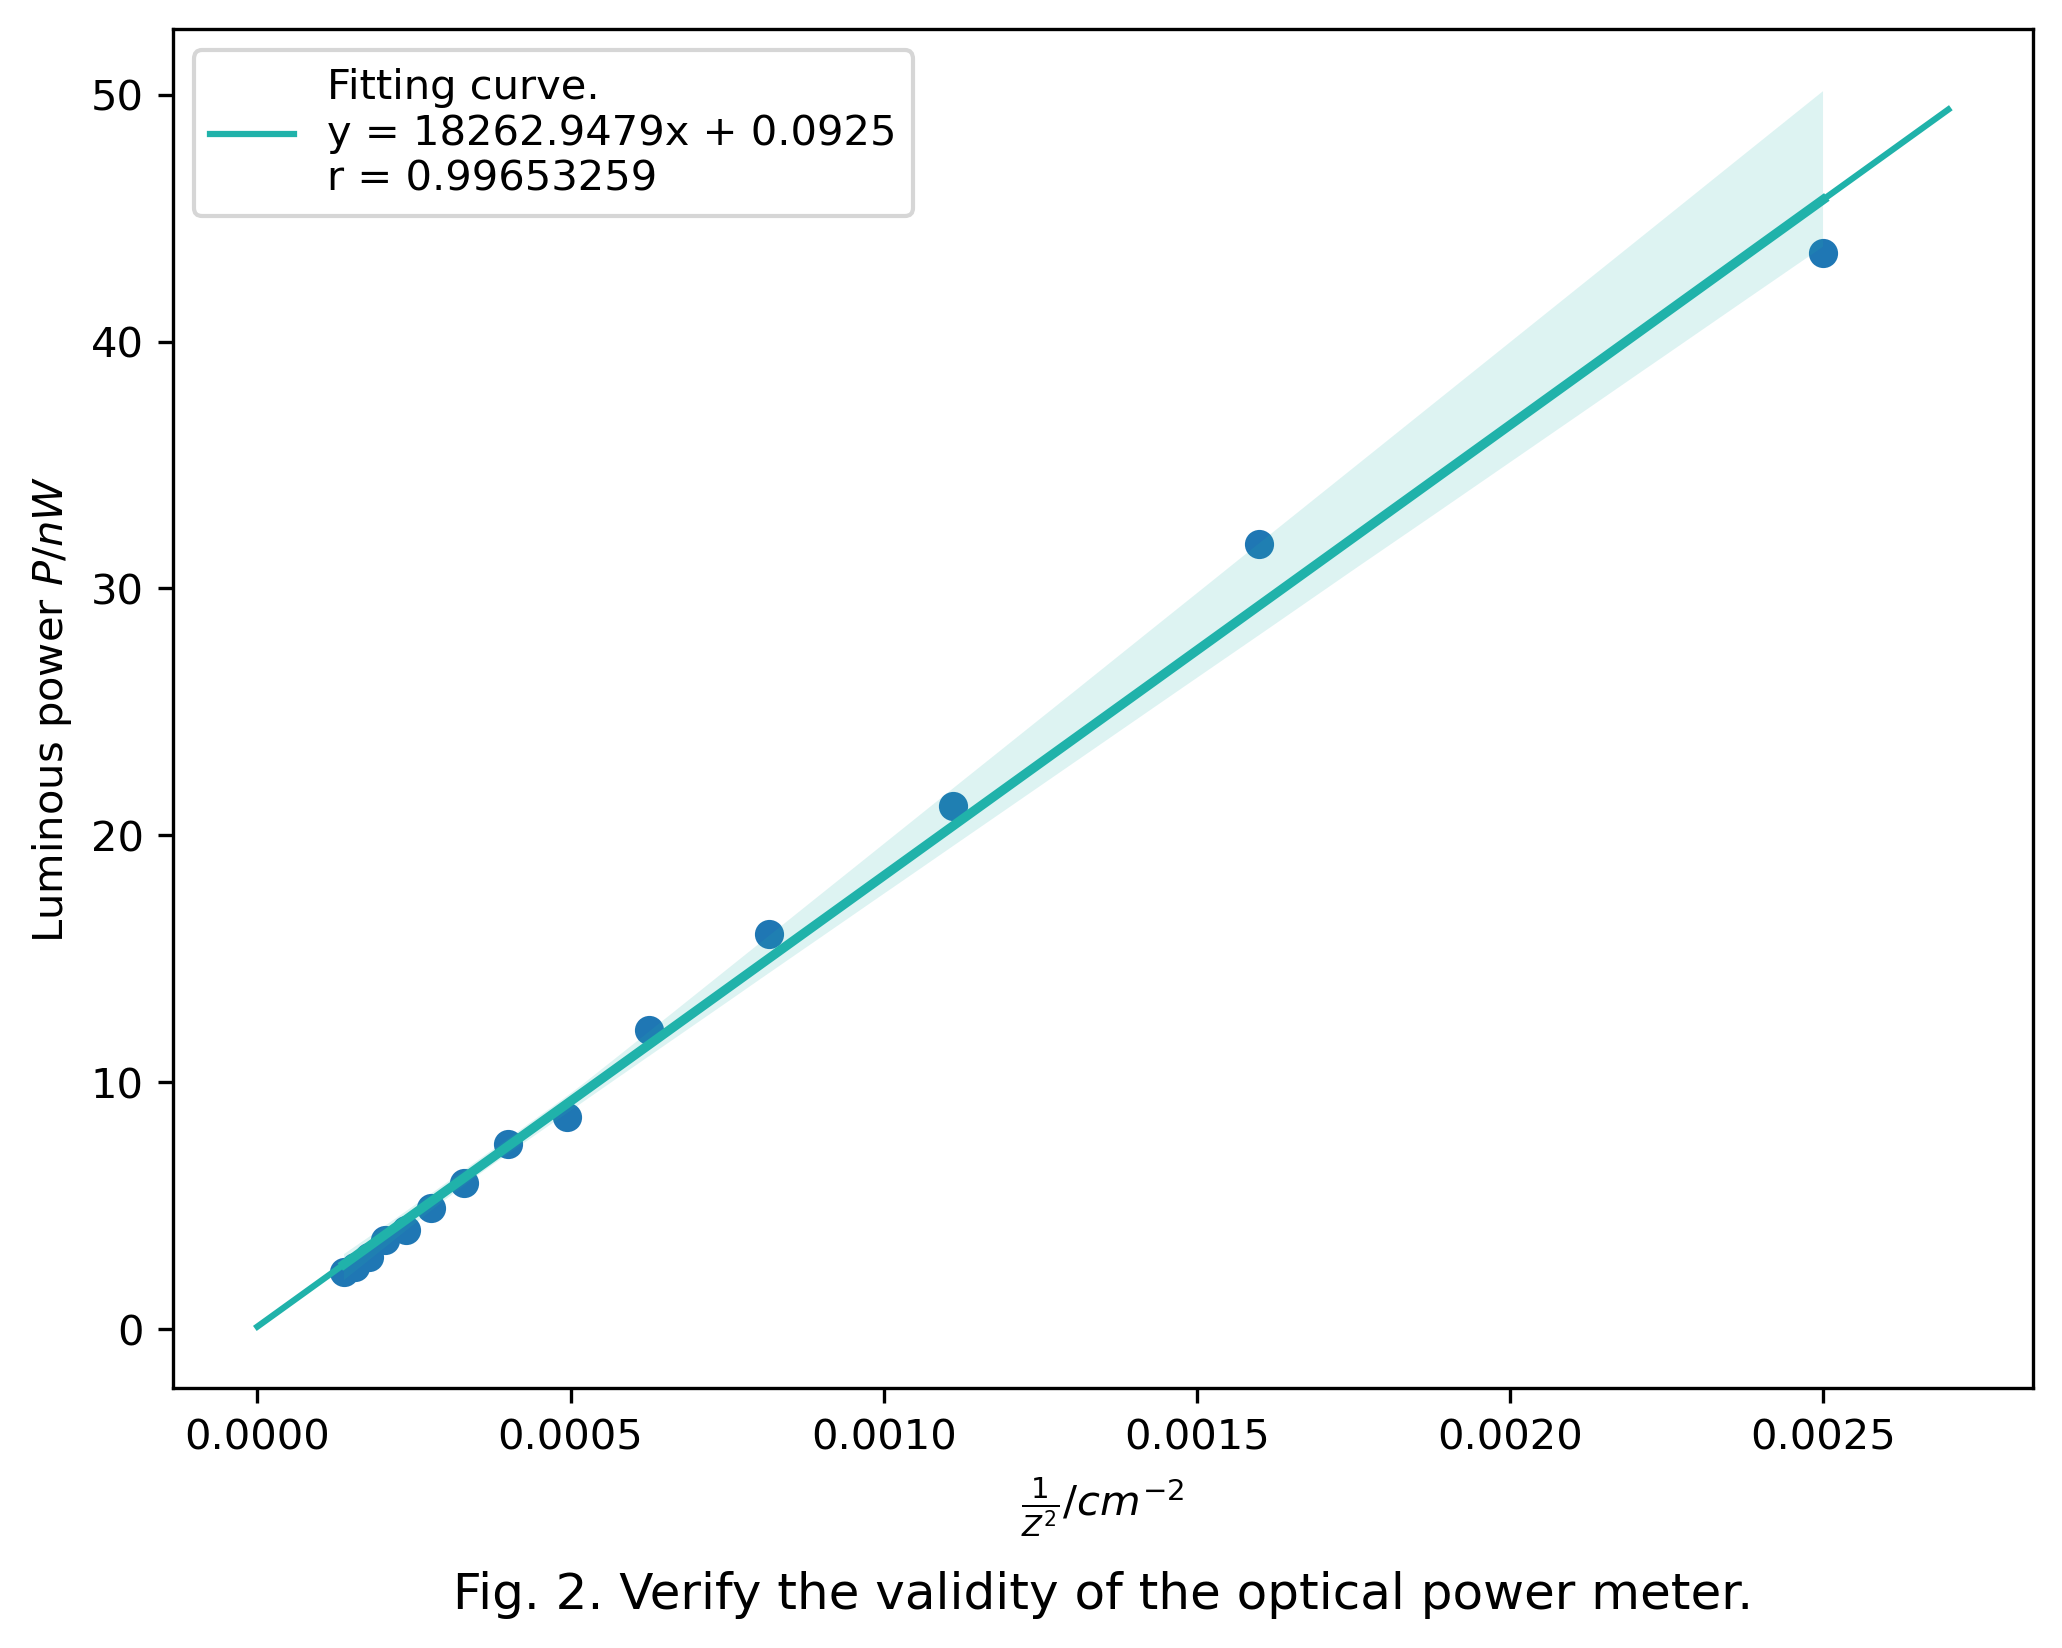
\includegraphics[width = 0.9\textwidth]{attachments//Fig.2.png}
	\caption{$P \sim \frac{1}{Z^2}$}
	\label{fig:2}
\end{minipage}
\end{figure}

\subsubsection*{3. $Seelight$仿真实验}
在$Seelight$光学仿真平台上搭建光路,采用与实验室实验相同的参数(表\ref{tab:0})进行仿真实验。
光路如\ref{fig:illus-3.1},仿真结果如\ref{fig:illus-3.2}

下载矩阵,使用seaborn重新绘制。我们注意到Seelight平台图像标度可能存在有误,
因此按照设定的屏尺寸$2cm \times 2cm$重新建立映射。结果如图\ref{fig:3.1}所示。
可以看出,衍射图样中光能量主要集中于主极大,次级大光强迅速衰减。

绘制相对光强分布,如图\ref{fig:3.2}。
对比仿真结果和理论曲线,我们发现零级主极大条纹光强分布与理论曲线符合较好,
但次级大相对光强偏低,且随着级次升高相对偏差越大,四级以及更高级次条纹消失。
条纹各次级大峰值与理论对照以及相对误差如表\ref{tab:3.1}。
($P_{the}$:理论光功率;$P_{exp}$:实验光功率;$I'_{the}$:理论相对光强;$I'_{exp}$:实验相对光强)

同时,我们测量了各次极大及各级暗纹的位置,结果如表\ref{tab:3.2}和表\ref{tab:3.3}。
实验值相对误差较小,与理论预测相符。
计算暗条纹间距均为$1.61mm$,与理论值$1.617mm$相比相对误差为$0.43\%$

\begin{figure}[htbp]
	\centering
	\subfloat[光路设置]{\label{fig:illus-3.1}
	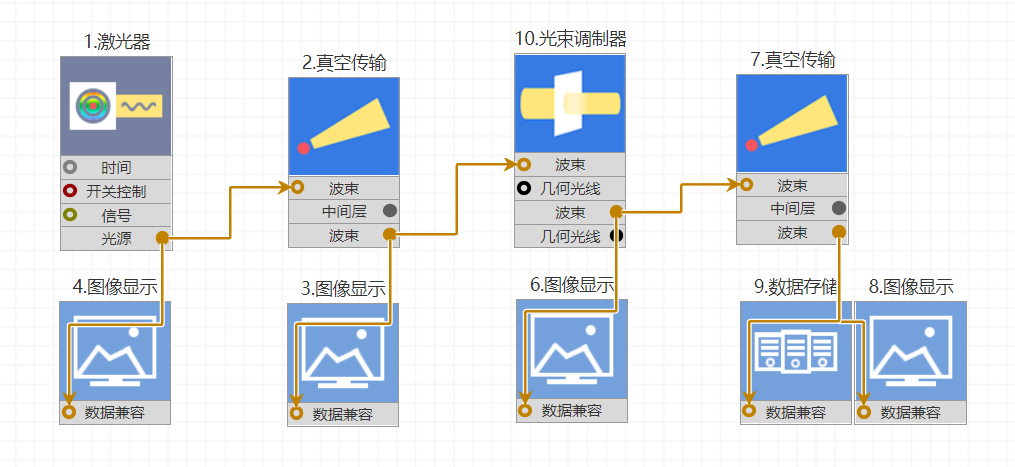
\includegraphics[height=5cm]{attachments/illus-3.1.png}
	}
	\subfloat[仿真结果]{\label{fig:illus-3.2}
	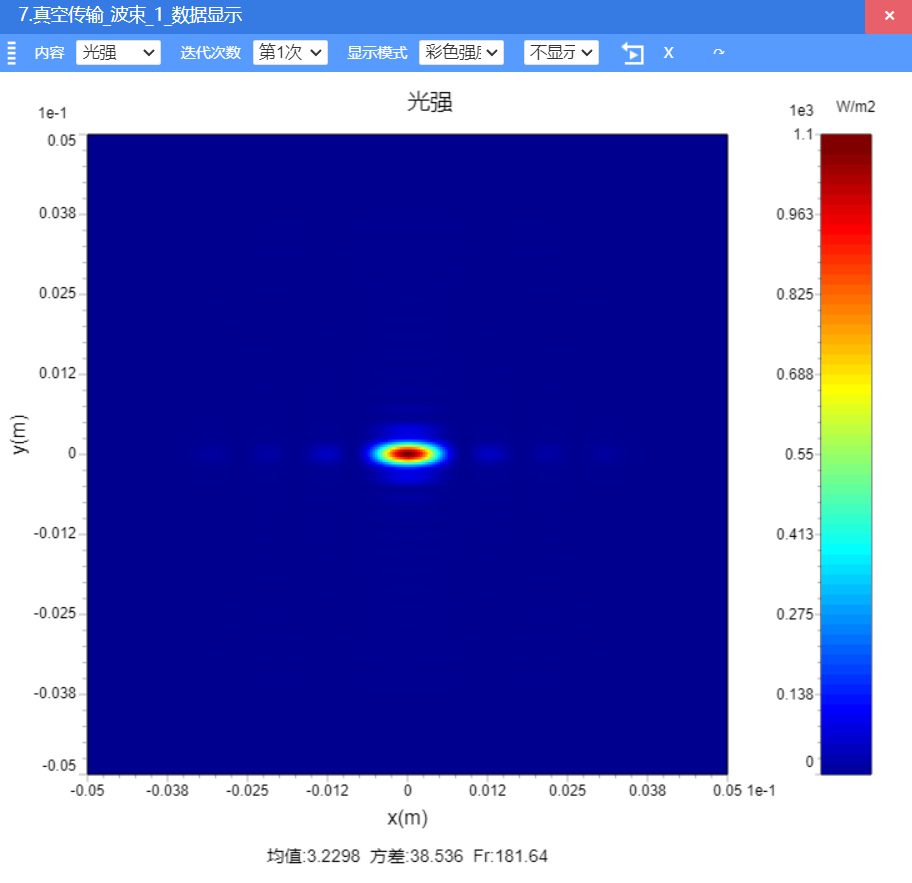
\includegraphics[height=5cm]{attachments/illus-3.2.png}
	}
	\caption{Seelight平台截图}
\end{figure}

\begin{figure}[htbp]
	\centering
	\subfloat[]{\label{fig:3.1.1}
	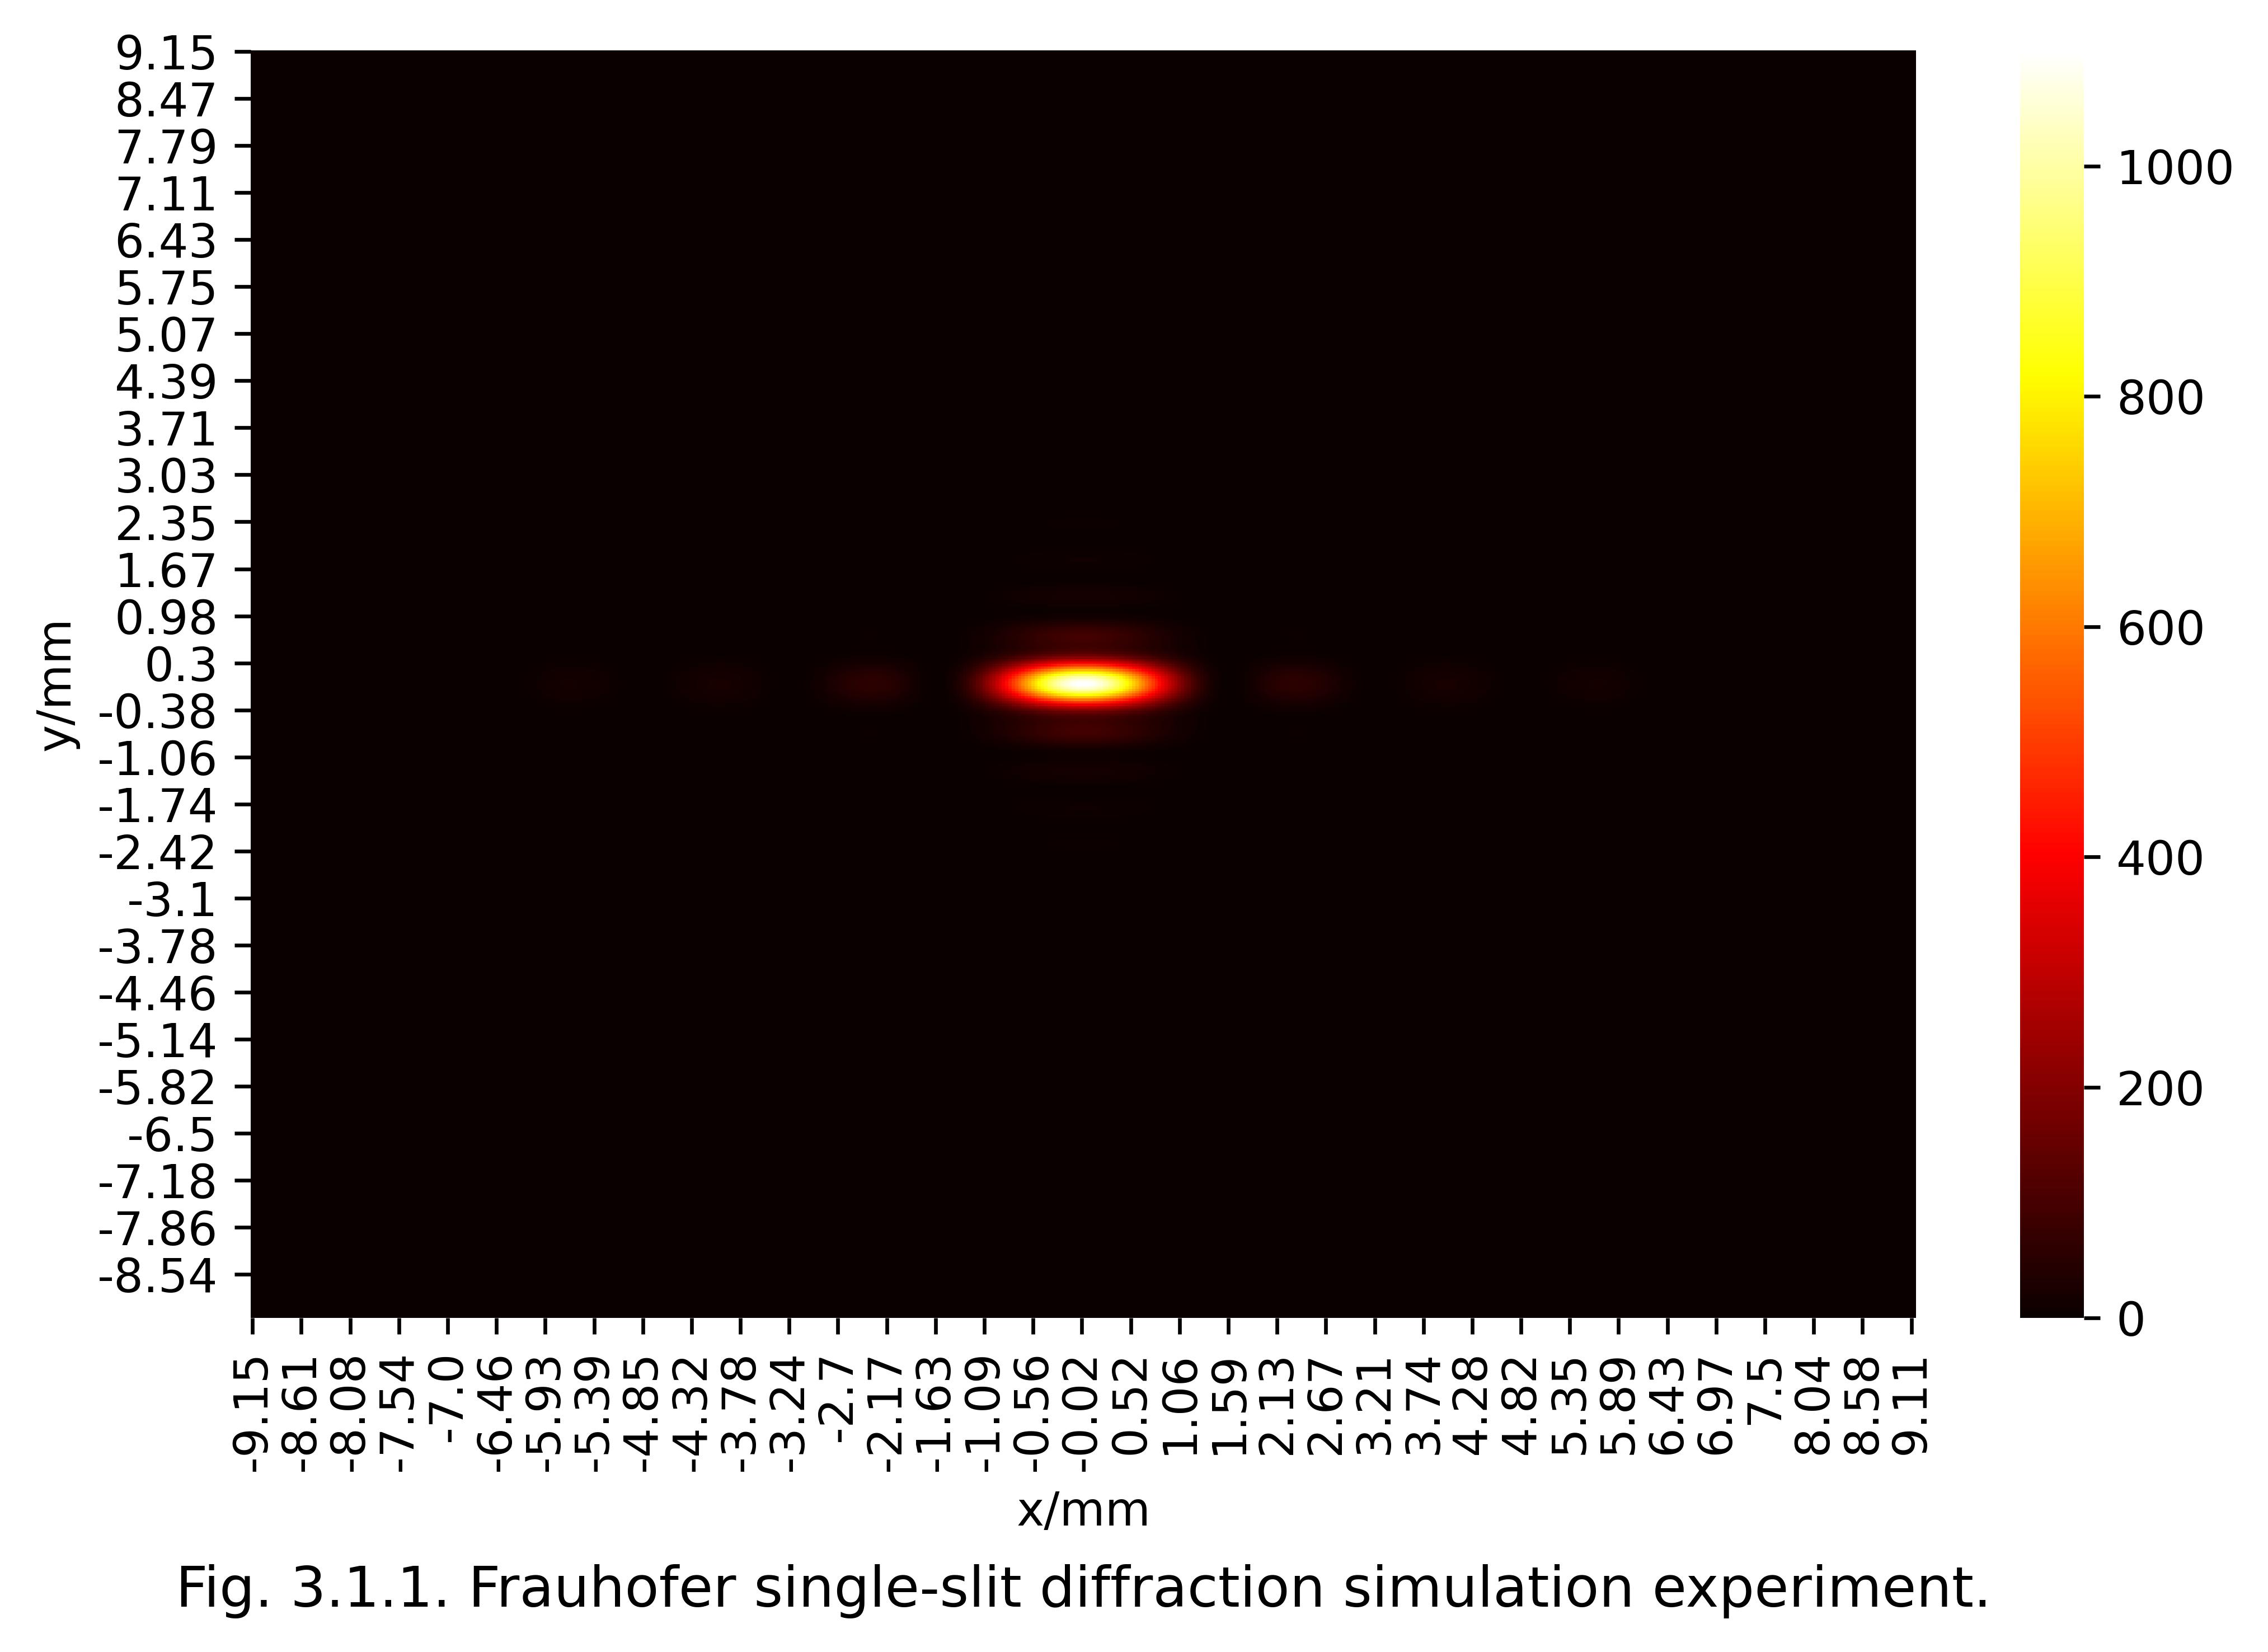
\includegraphics[width=0.5\textwidth]{attachments/Fig.3.1.1.png}
	}
	\subfloat[]{\label{fig:3.1.2}
	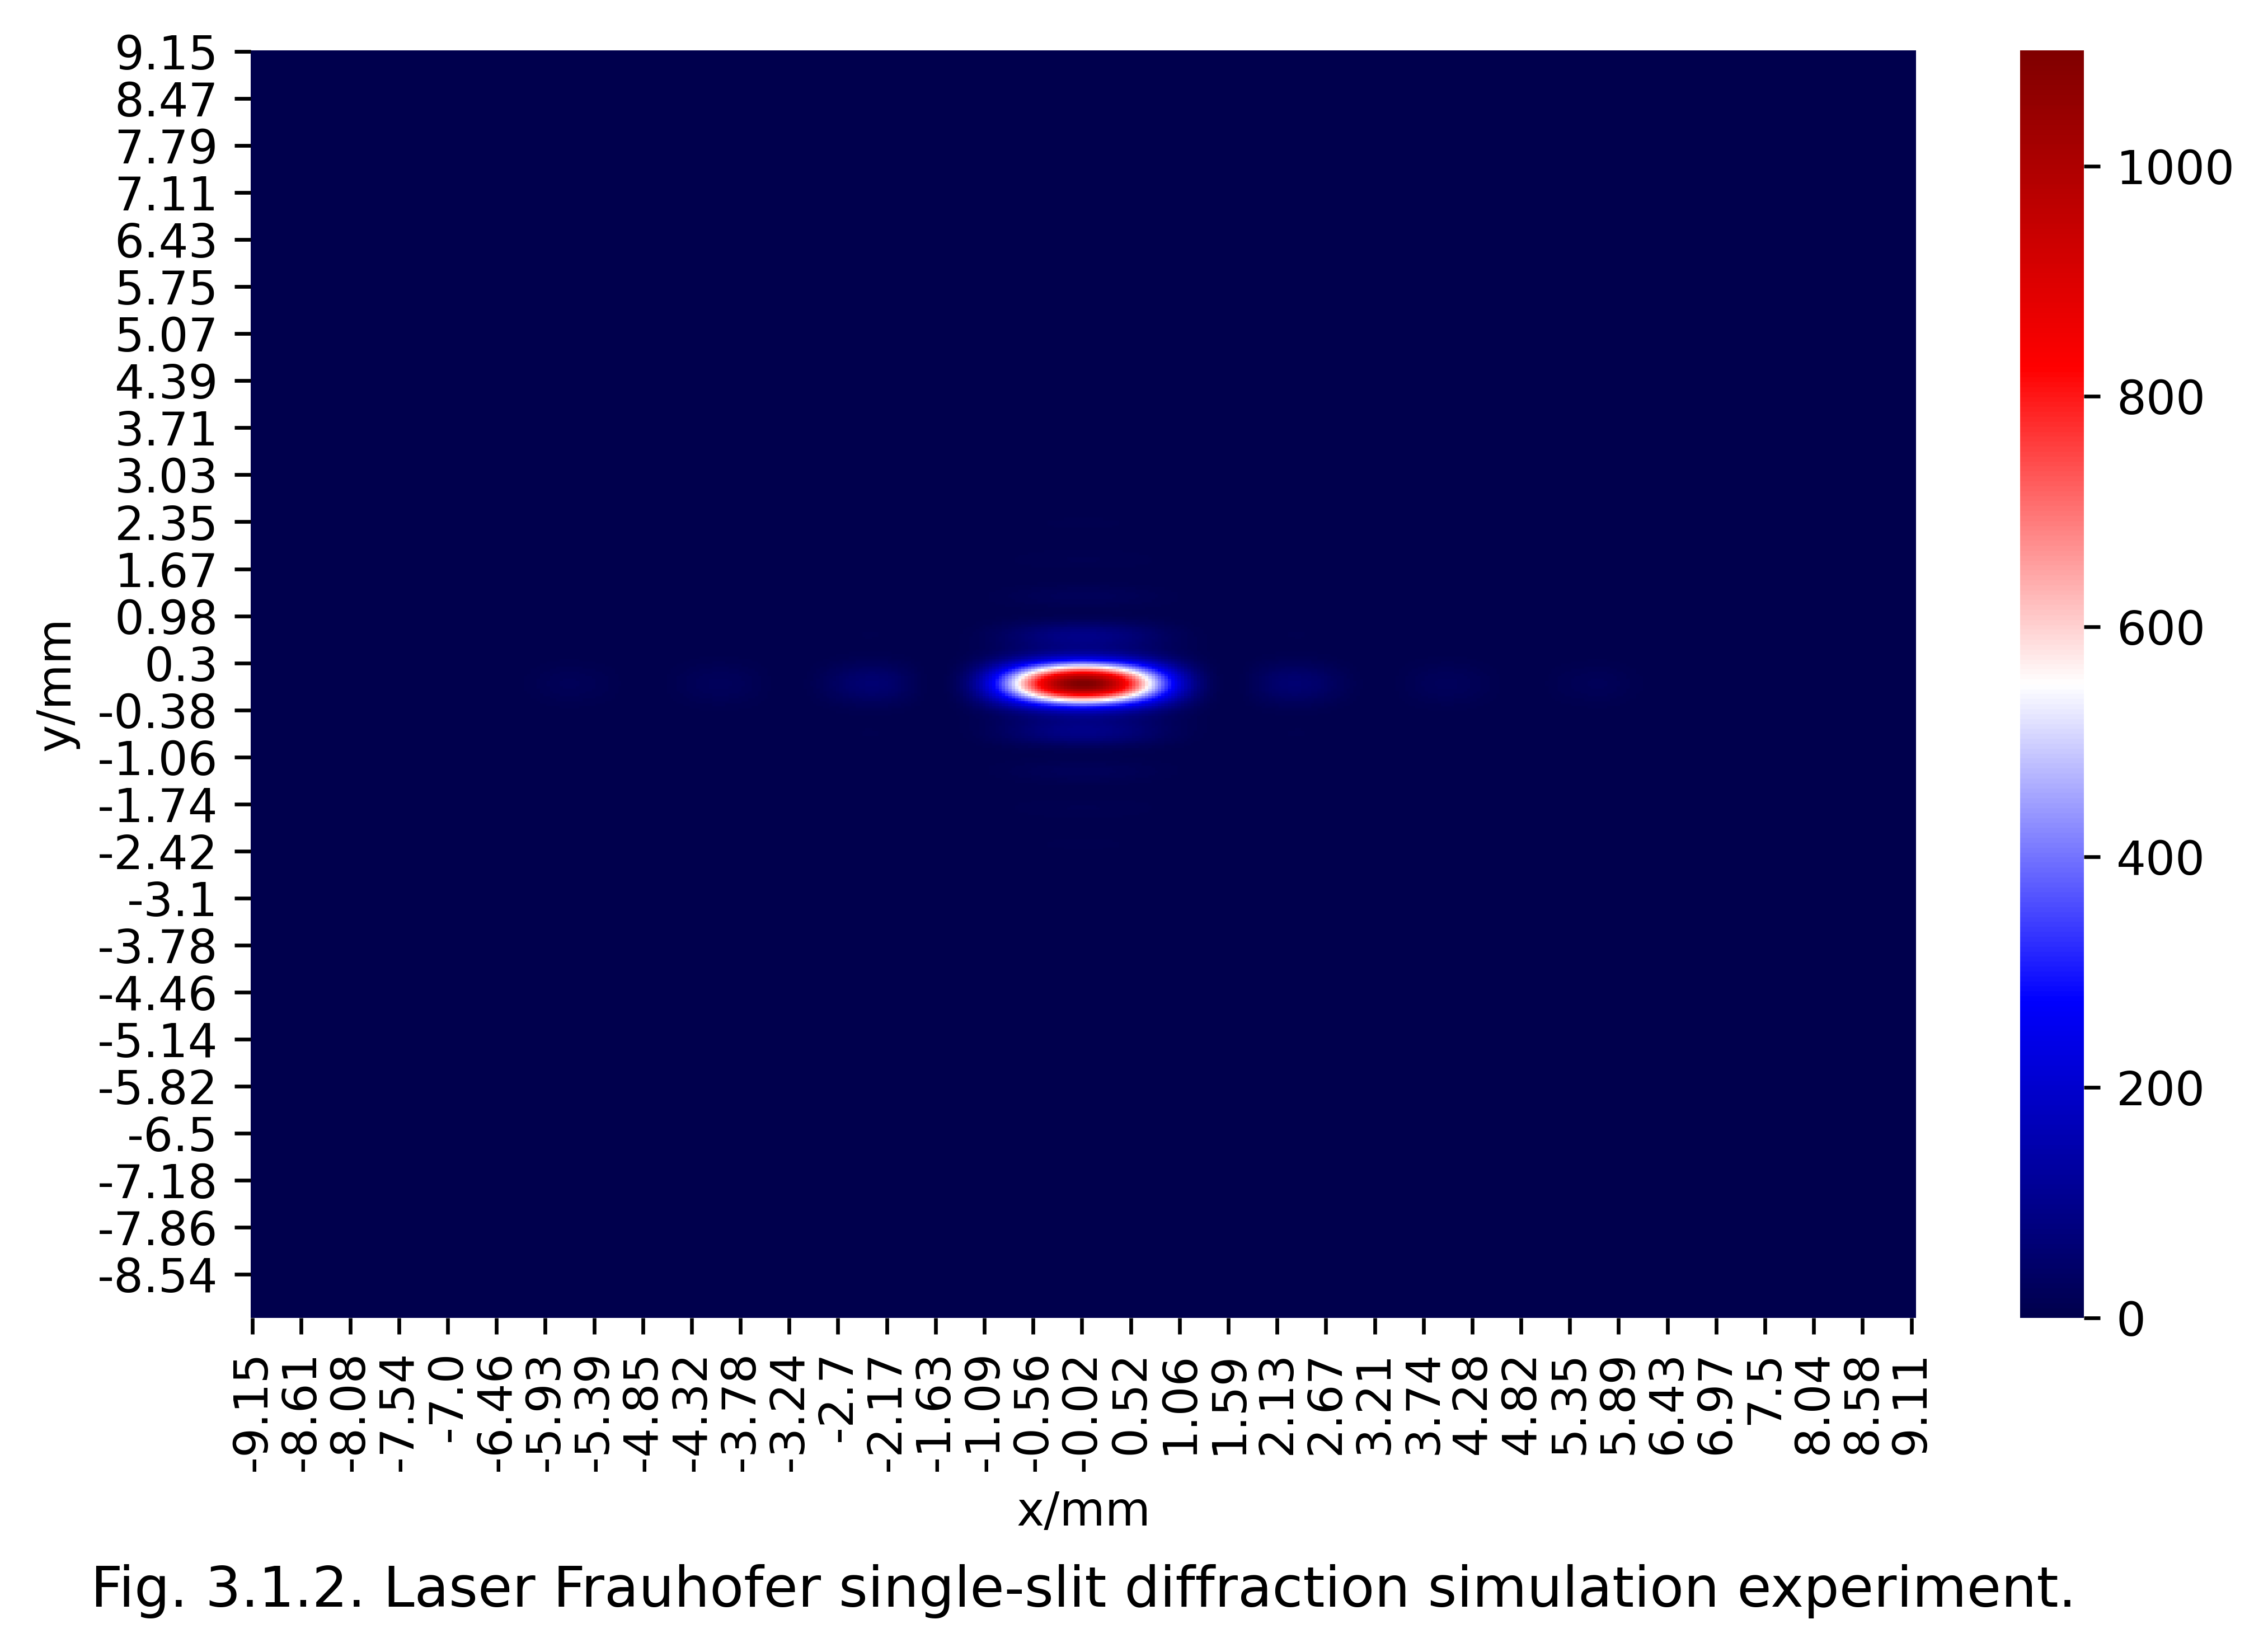
\includegraphics[width=0.5\textwidth]{attachments/Fig.3.1.2.png}
	}
	\caption{仿真衍射图样}
	\label{fig:3.1}
\end{figure}

\begin{figure}[htbp]
	\centering
	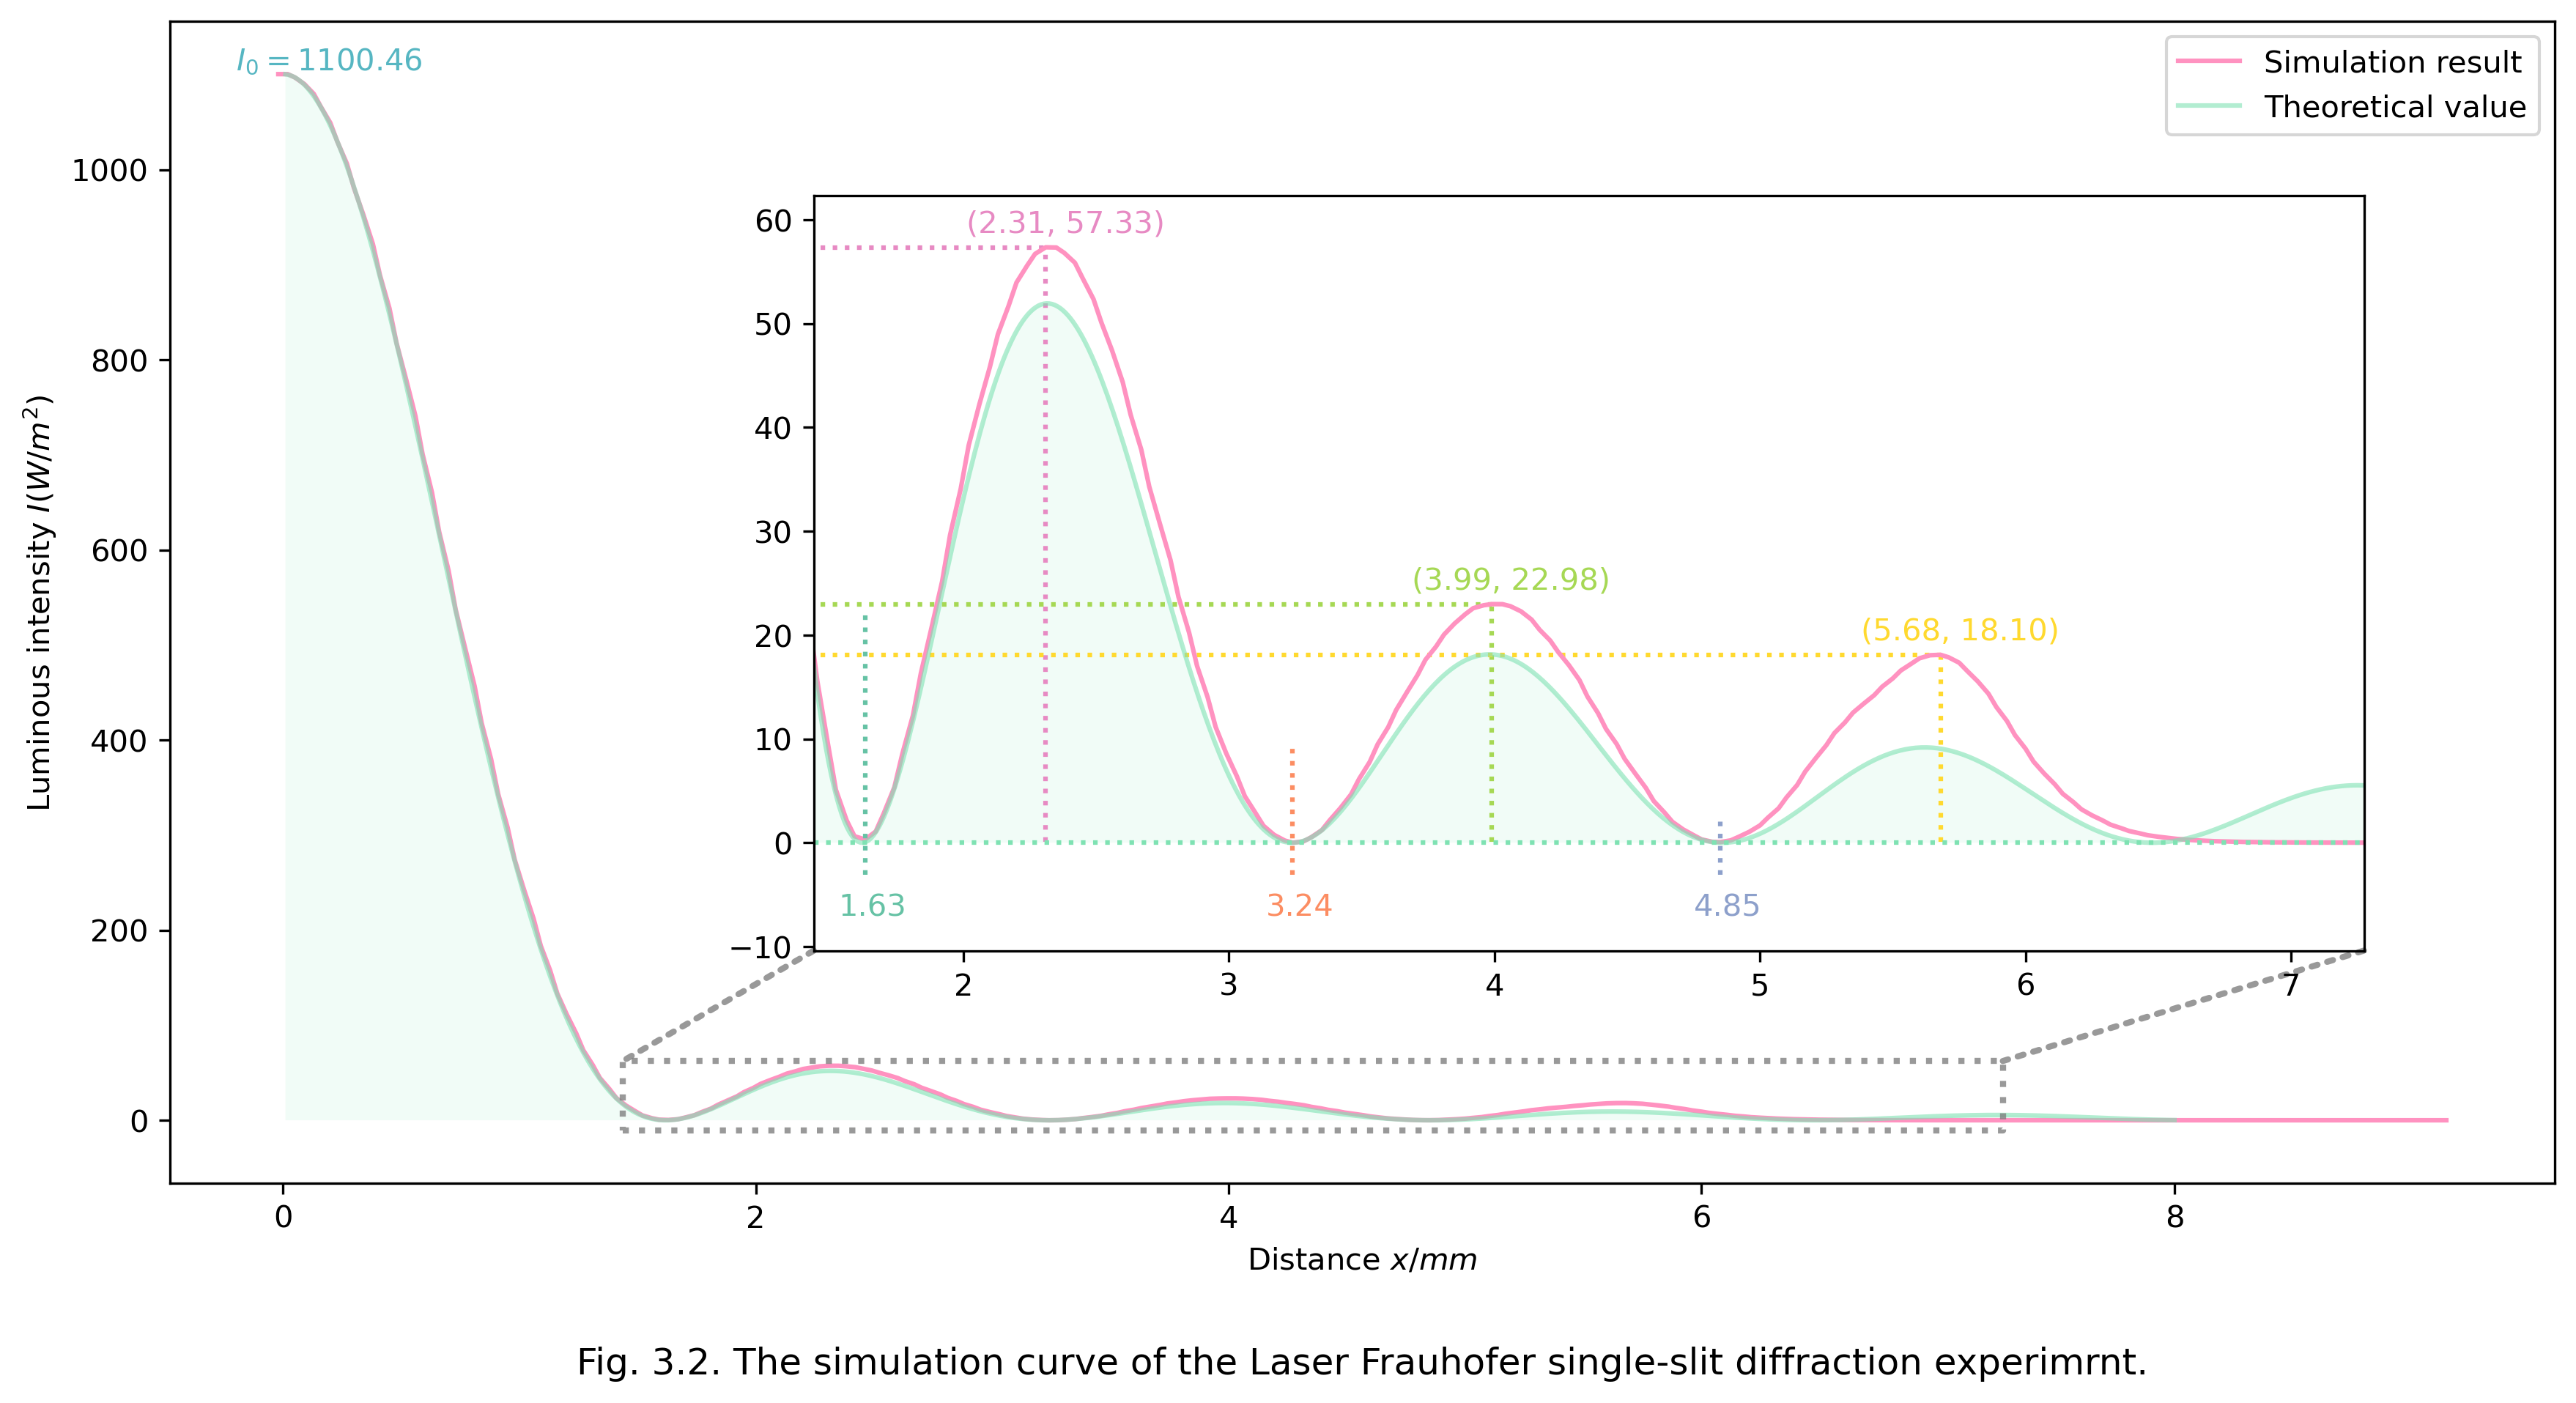
\includegraphics[width=0.8\textwidth]{attachments//Fig.3.2.png}
	\caption{仿真曲线}
	\label{fig:3.2}
\end{figure}

\begin{table}[htbp]
	\centering
	\begin{tabular}{cccccc}
	\toprule
	条纹级次 &$P_{the}/nW$ &$P_{exp}/nW$ &$I'_{the}$ &$I'_{exp}$ &相对误差 \\
	\midrule
	1  &51.930763  &57.334587  &0.047190  &0.052101  &-10.41\%	\\	
	2  &18.132388  &22.977563  &0.016477  &0.020880  &-26.72\%	\\
	3  & 9.170325  &18.096673  &0.008333  &0.016445  &-97.34\%	\\
	\bottomrule
    \end{tabular}
	\caption{\textbf{次级大条纹峰值}}
	\label{tab:3.1}
\end{table}


\begin{table}[htbp]
	\centering
		\begin{tabular}{cccc}
			\toprule
			条纹级次	&理论位置$/mm$	&实验位置$/mm$	&相对误差 \\
			\midrule
			1  &2.313  &2.31  &0.12\% \\
			2  &3.985  &3.99  &-0.13\% \\
			3  &5.617  &5.68  &-1.12\% \\	
			\bottomrule
		\end{tabular}
		\caption{\textbf{次级大条纹位置}}
		\label{tab:3.2}
\end{table}
\begin{table}[htbp]
	\centering
		\begin{tabular}{cccc}
			\toprule
			条纹级次	&理论位置$/mm$	&实验位置$/mm$	&相对误差 \\
			\midrule
			1  &1.622  &1.63  &-0.49\% \\
			2  &3.234  &3.24   &-0.18\% \\
			3  &4.856  &4.85   &0.13\% \\	
			\bottomrule
		\end{tabular}
		\caption{\textbf{暗纹位置}}
		\label{tab:3.3}
\end{table}

\newpage
\subsection*{【思考题】}
\subsubsection*{1. 缝宽加倍或减半对衍射条纹的光强和宽度影响?}
答:根据式\ref{eq:1.5},缝宽增加一倍时,衍射条纹宽度增大,每条条纹上能量趋于分散,各级条纹光强极大值会减小。
与之相反,缝宽减半时,衍射条纹宽度减小,每条条纹上能量趋于集中,各级条纹光强极大值会增大。
\subsubsection*{2. 使用光功率计注意事项;光功率计进光狭缝宽度对实验影响。}
答:
\begin{enumerate}[label=\arabic*.]
	\item 使用光功率计时光探头应尽量正对入射光线。实验时应精细调节底座,使光功率计示数最大时再进行读数。此外,测量过程中应尽量避免周围有较亮光源。同时,要注意保证光功率计工作在线性区。	
	\item 进光狭缝宽度窄,能采集到近似一点处光强,测量精度更高,避免周围光源影响。但当狭缝过窄以致入射光光强过小时,可能会受光功率计本身测量精度限制而读数变化不大。
\end{enumerate}
\subsubsection*{3. 检查光功率计是否工作在线性区时,能否采用激光光源。}
答:不能。激光能量集中,光强大,容易超出光功率计的线性工作区。
\subsubsection*{4. 证明本实验能满足夫琅禾费衍射条件}
将表\ref{tab:0}参数代入式\ref{eq:t1}检查得满足远距离条件。
\begin{equation}\label{eq:t1}
	\frac{a^2}{8Z\lambda} = 0.026 \ll 1
\end{equation}
\subsubsection*{5. 作出单缝,双缝,三缝,四缝,多缝透射光栅相对光强分布。}
多缝透射光栅衍射光强分布如式\ref{eq:t2}
\begin{equation}\label{eq:t2}
	I_N = I_0\frac{sin^2(\frac{\pi asin \theta}{\lambda})}{(\frac{\pi asin \theta}{\lambda})^2} \times \frac{sin^2(\frac{N\pi dsin \theta}{\lambda})}{sin^2(\frac{\pi dsin \theta}{\lambda})}
\end{equation}
采用表\ref{tab:0}参数,代入$N = 1,2,3,4,100$计算相对光强,绘制图线如\ref{fig:4}
\newpage
\begin{figure}[htbp]
	\centering
	\subfloat[N=1]{\label{fig:4.1}
	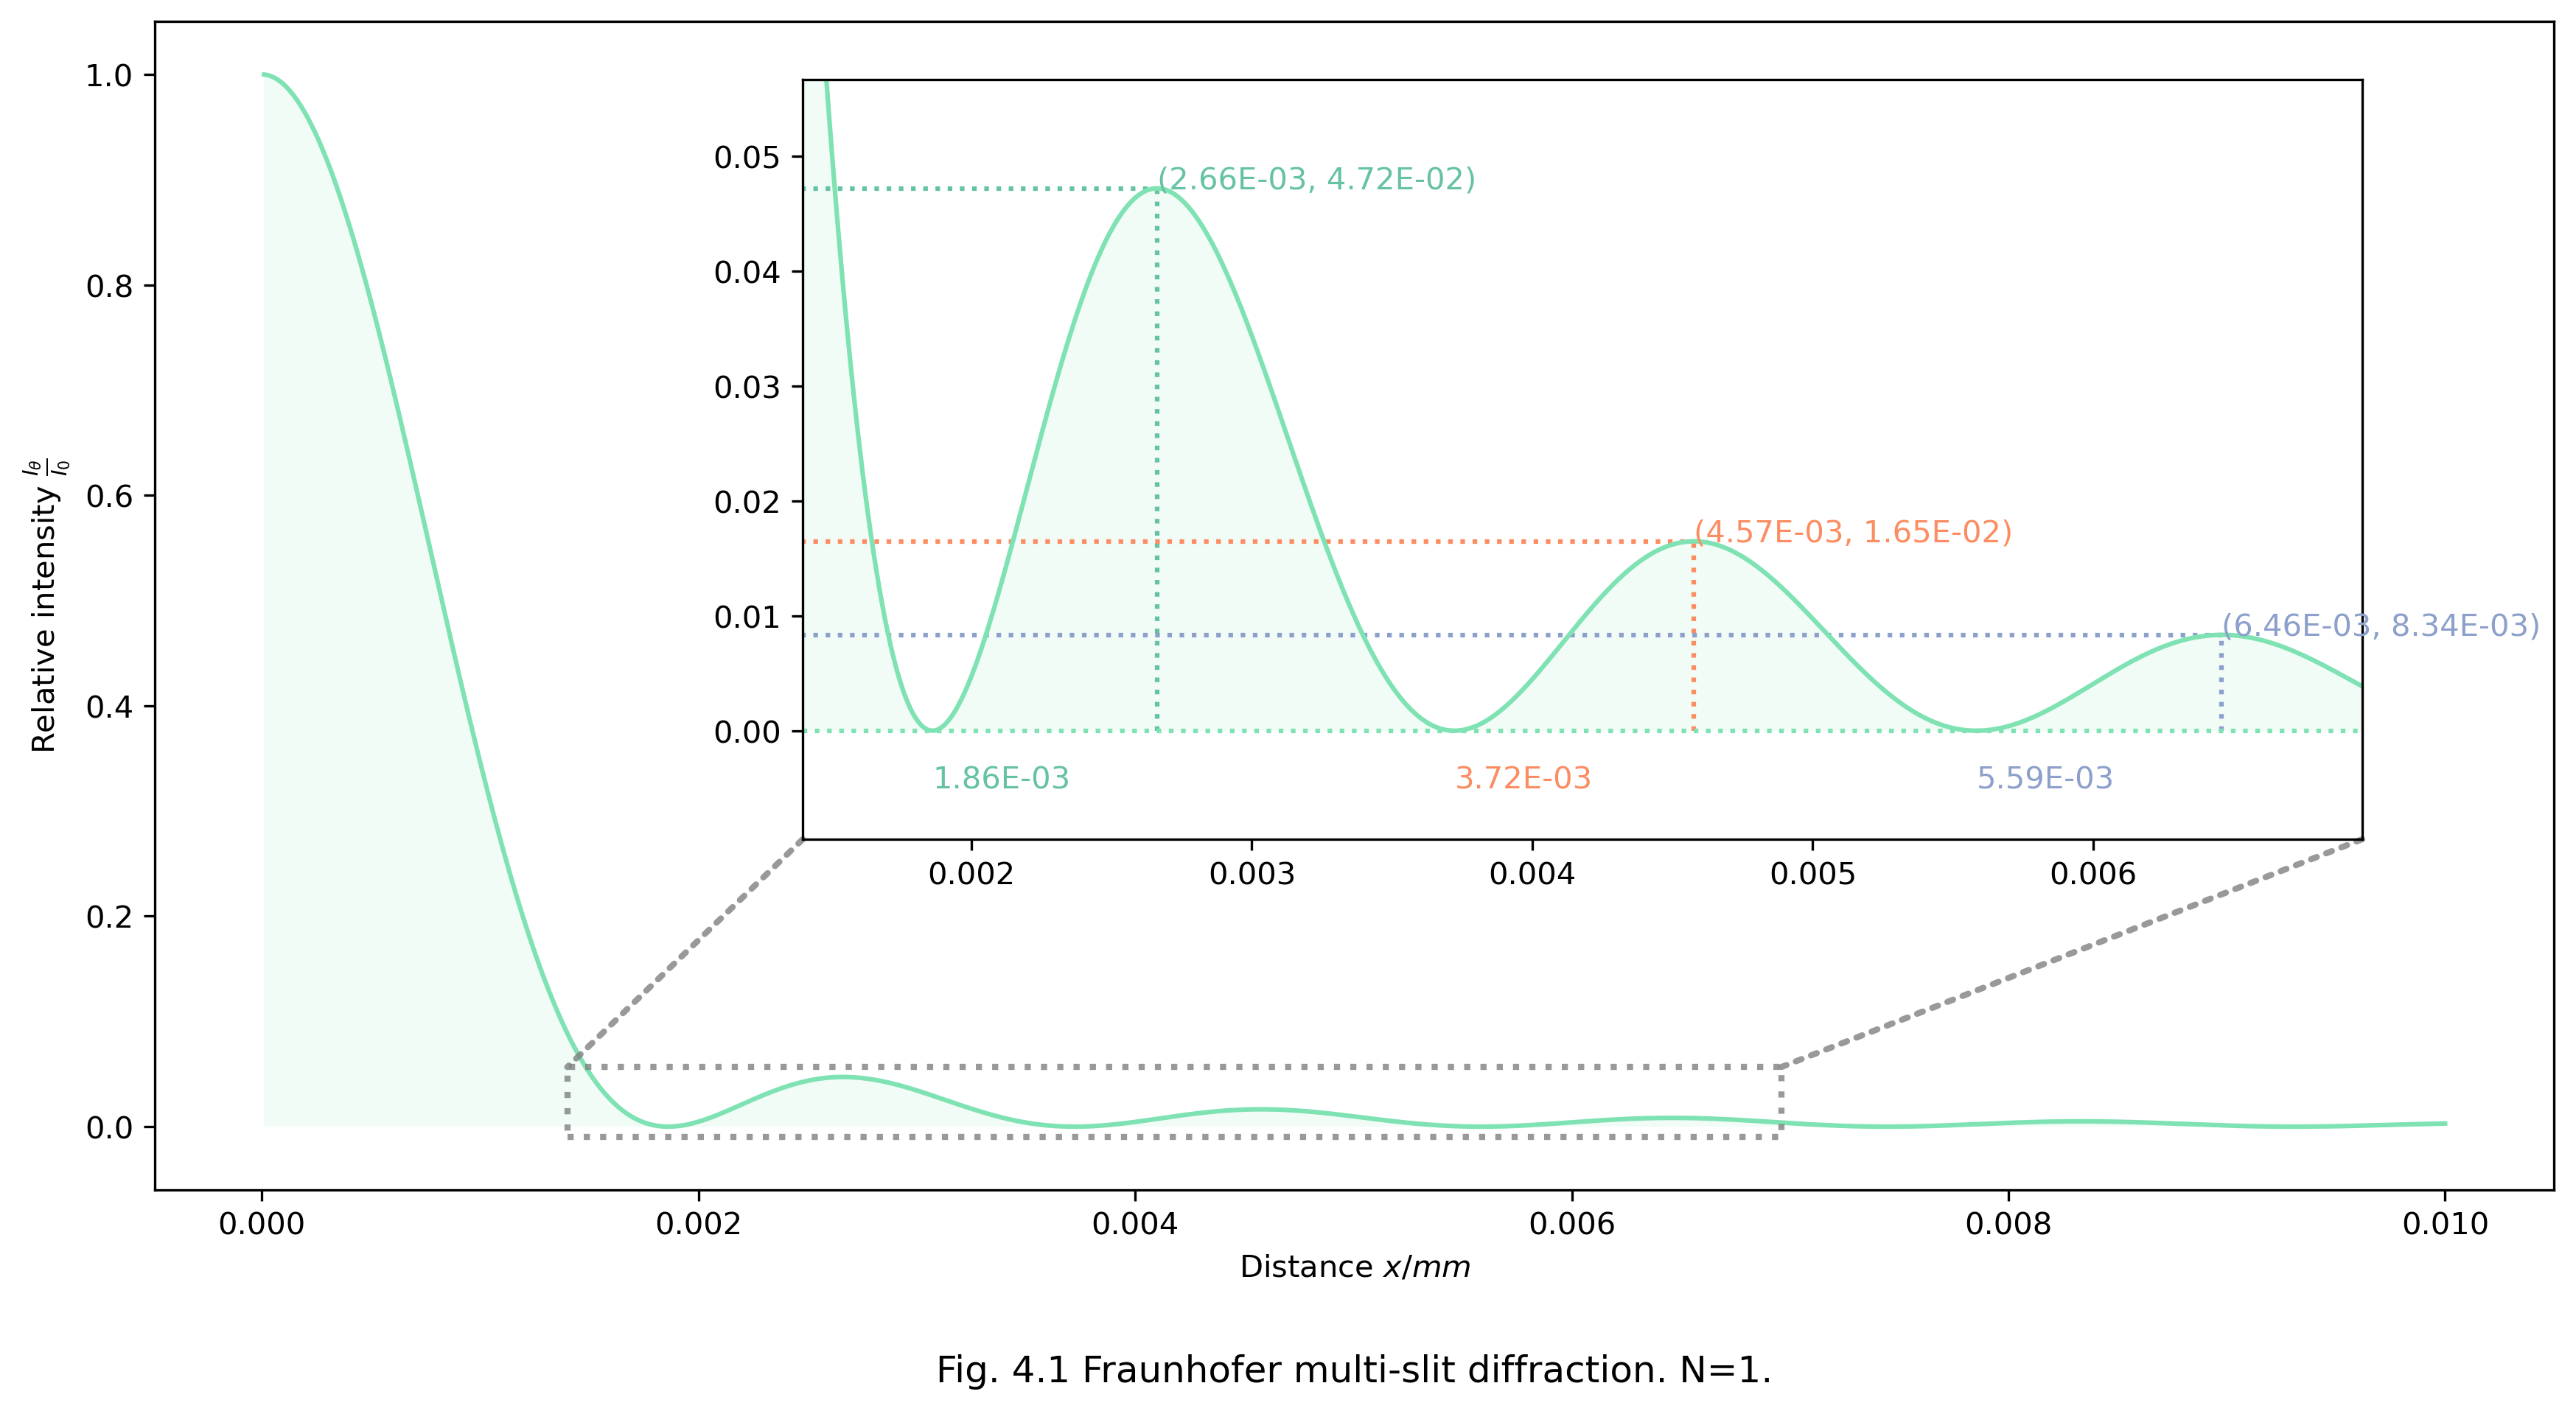
\includegraphics[width=0.5\textwidth]{attachments//Fig.4.1.png}
	}
	\subfloat[N=2]{\label{fig:4.2}
	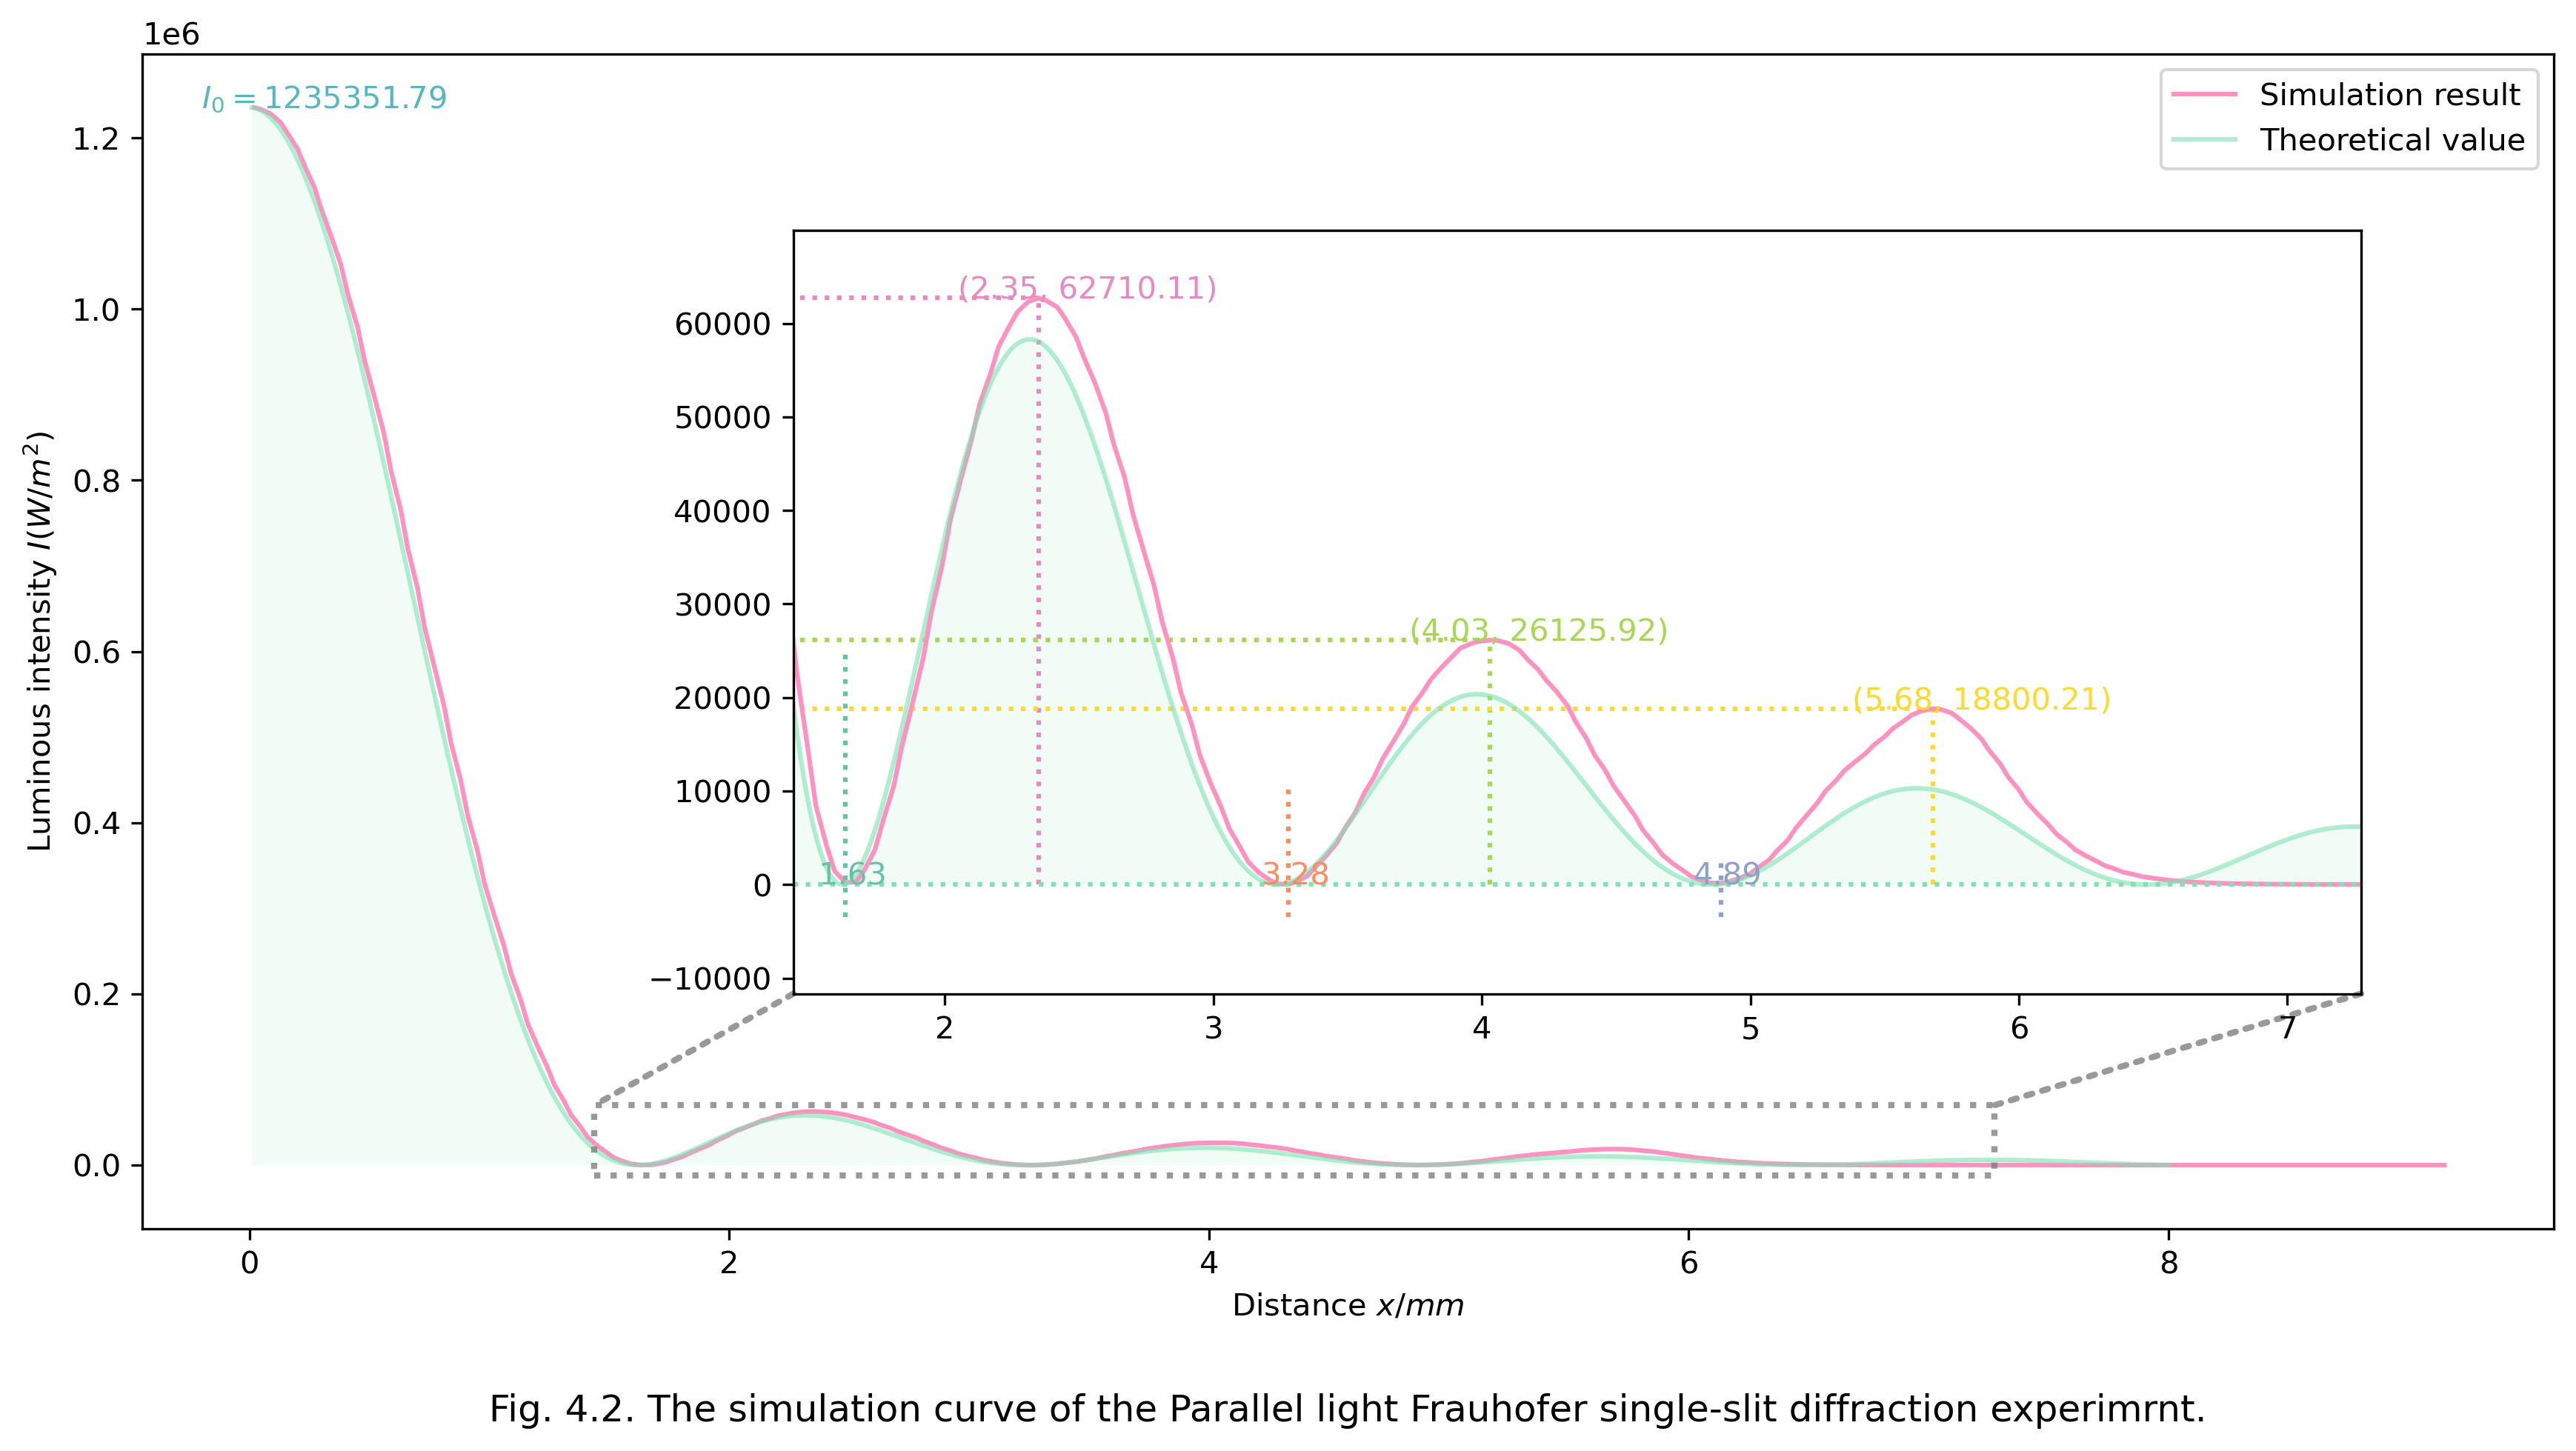
\includegraphics[width=0.5\textwidth]{attachments//Fig.4.2.png}
	}

	\subfloat[N=3]{\label{fig:4.3}
	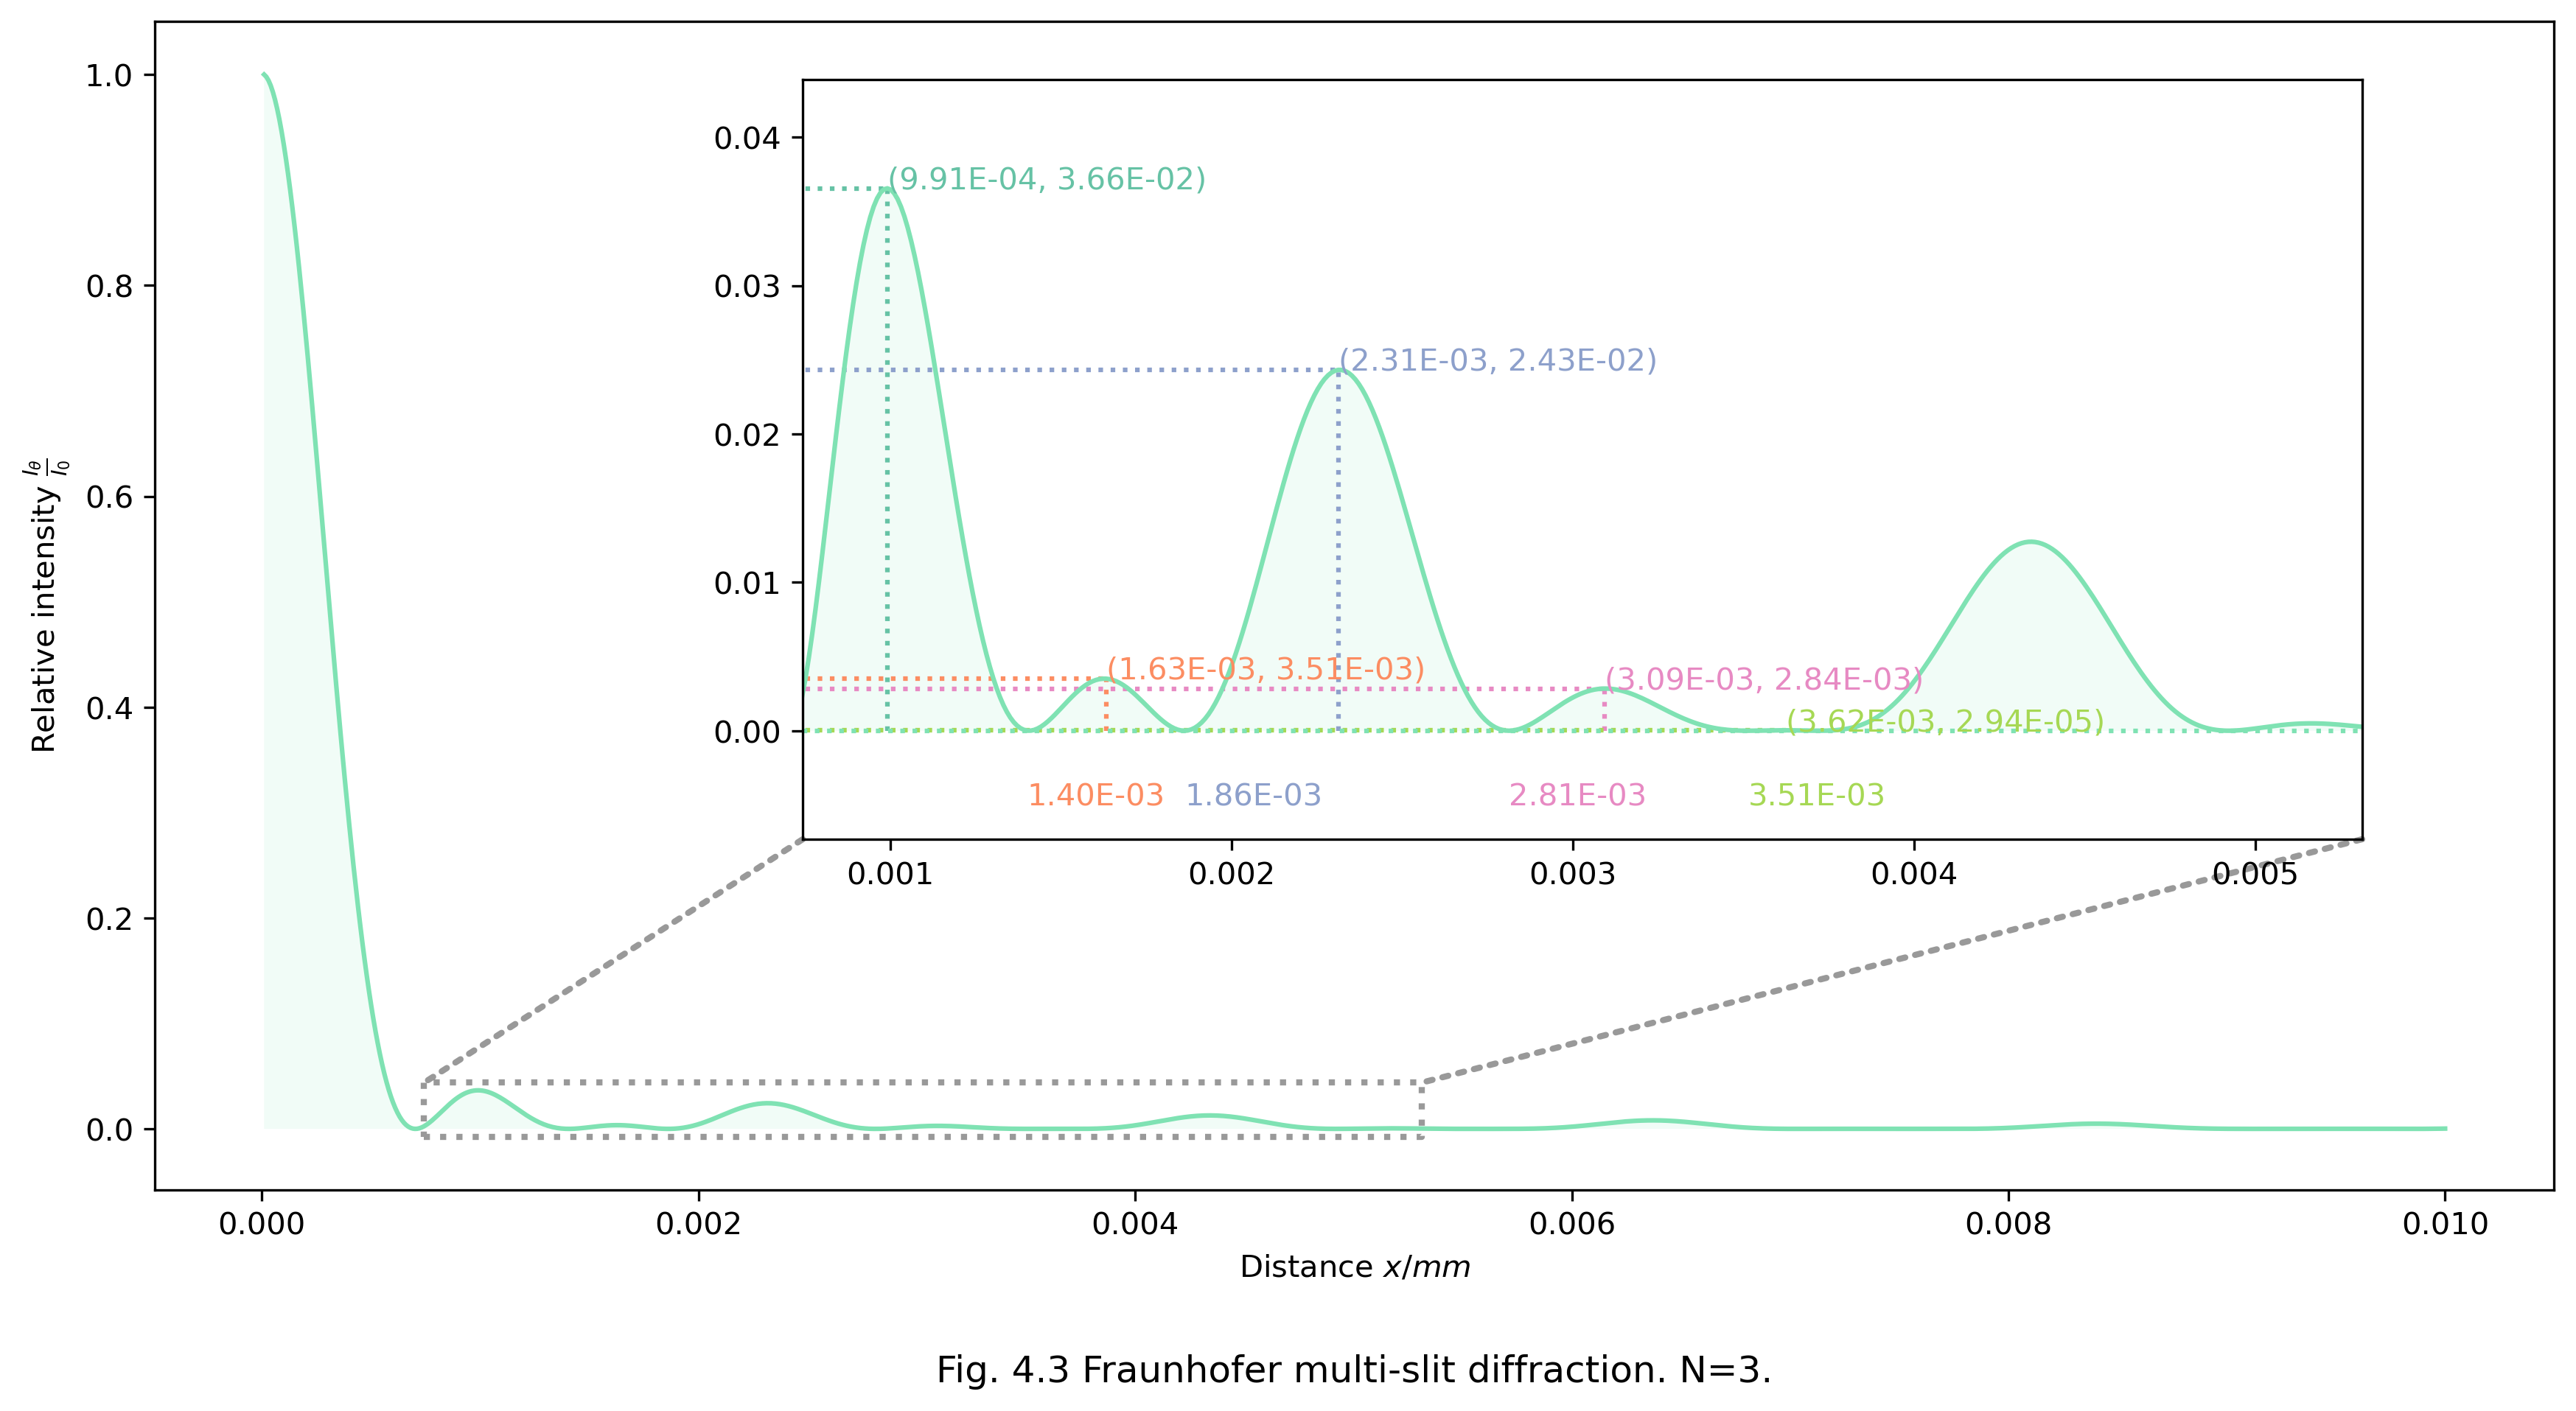
\includegraphics[width=0.5\textwidth]{attachments//Fig.4.3.png}
	}
	\subfloat[N=4]{\label{fig:4.4}
	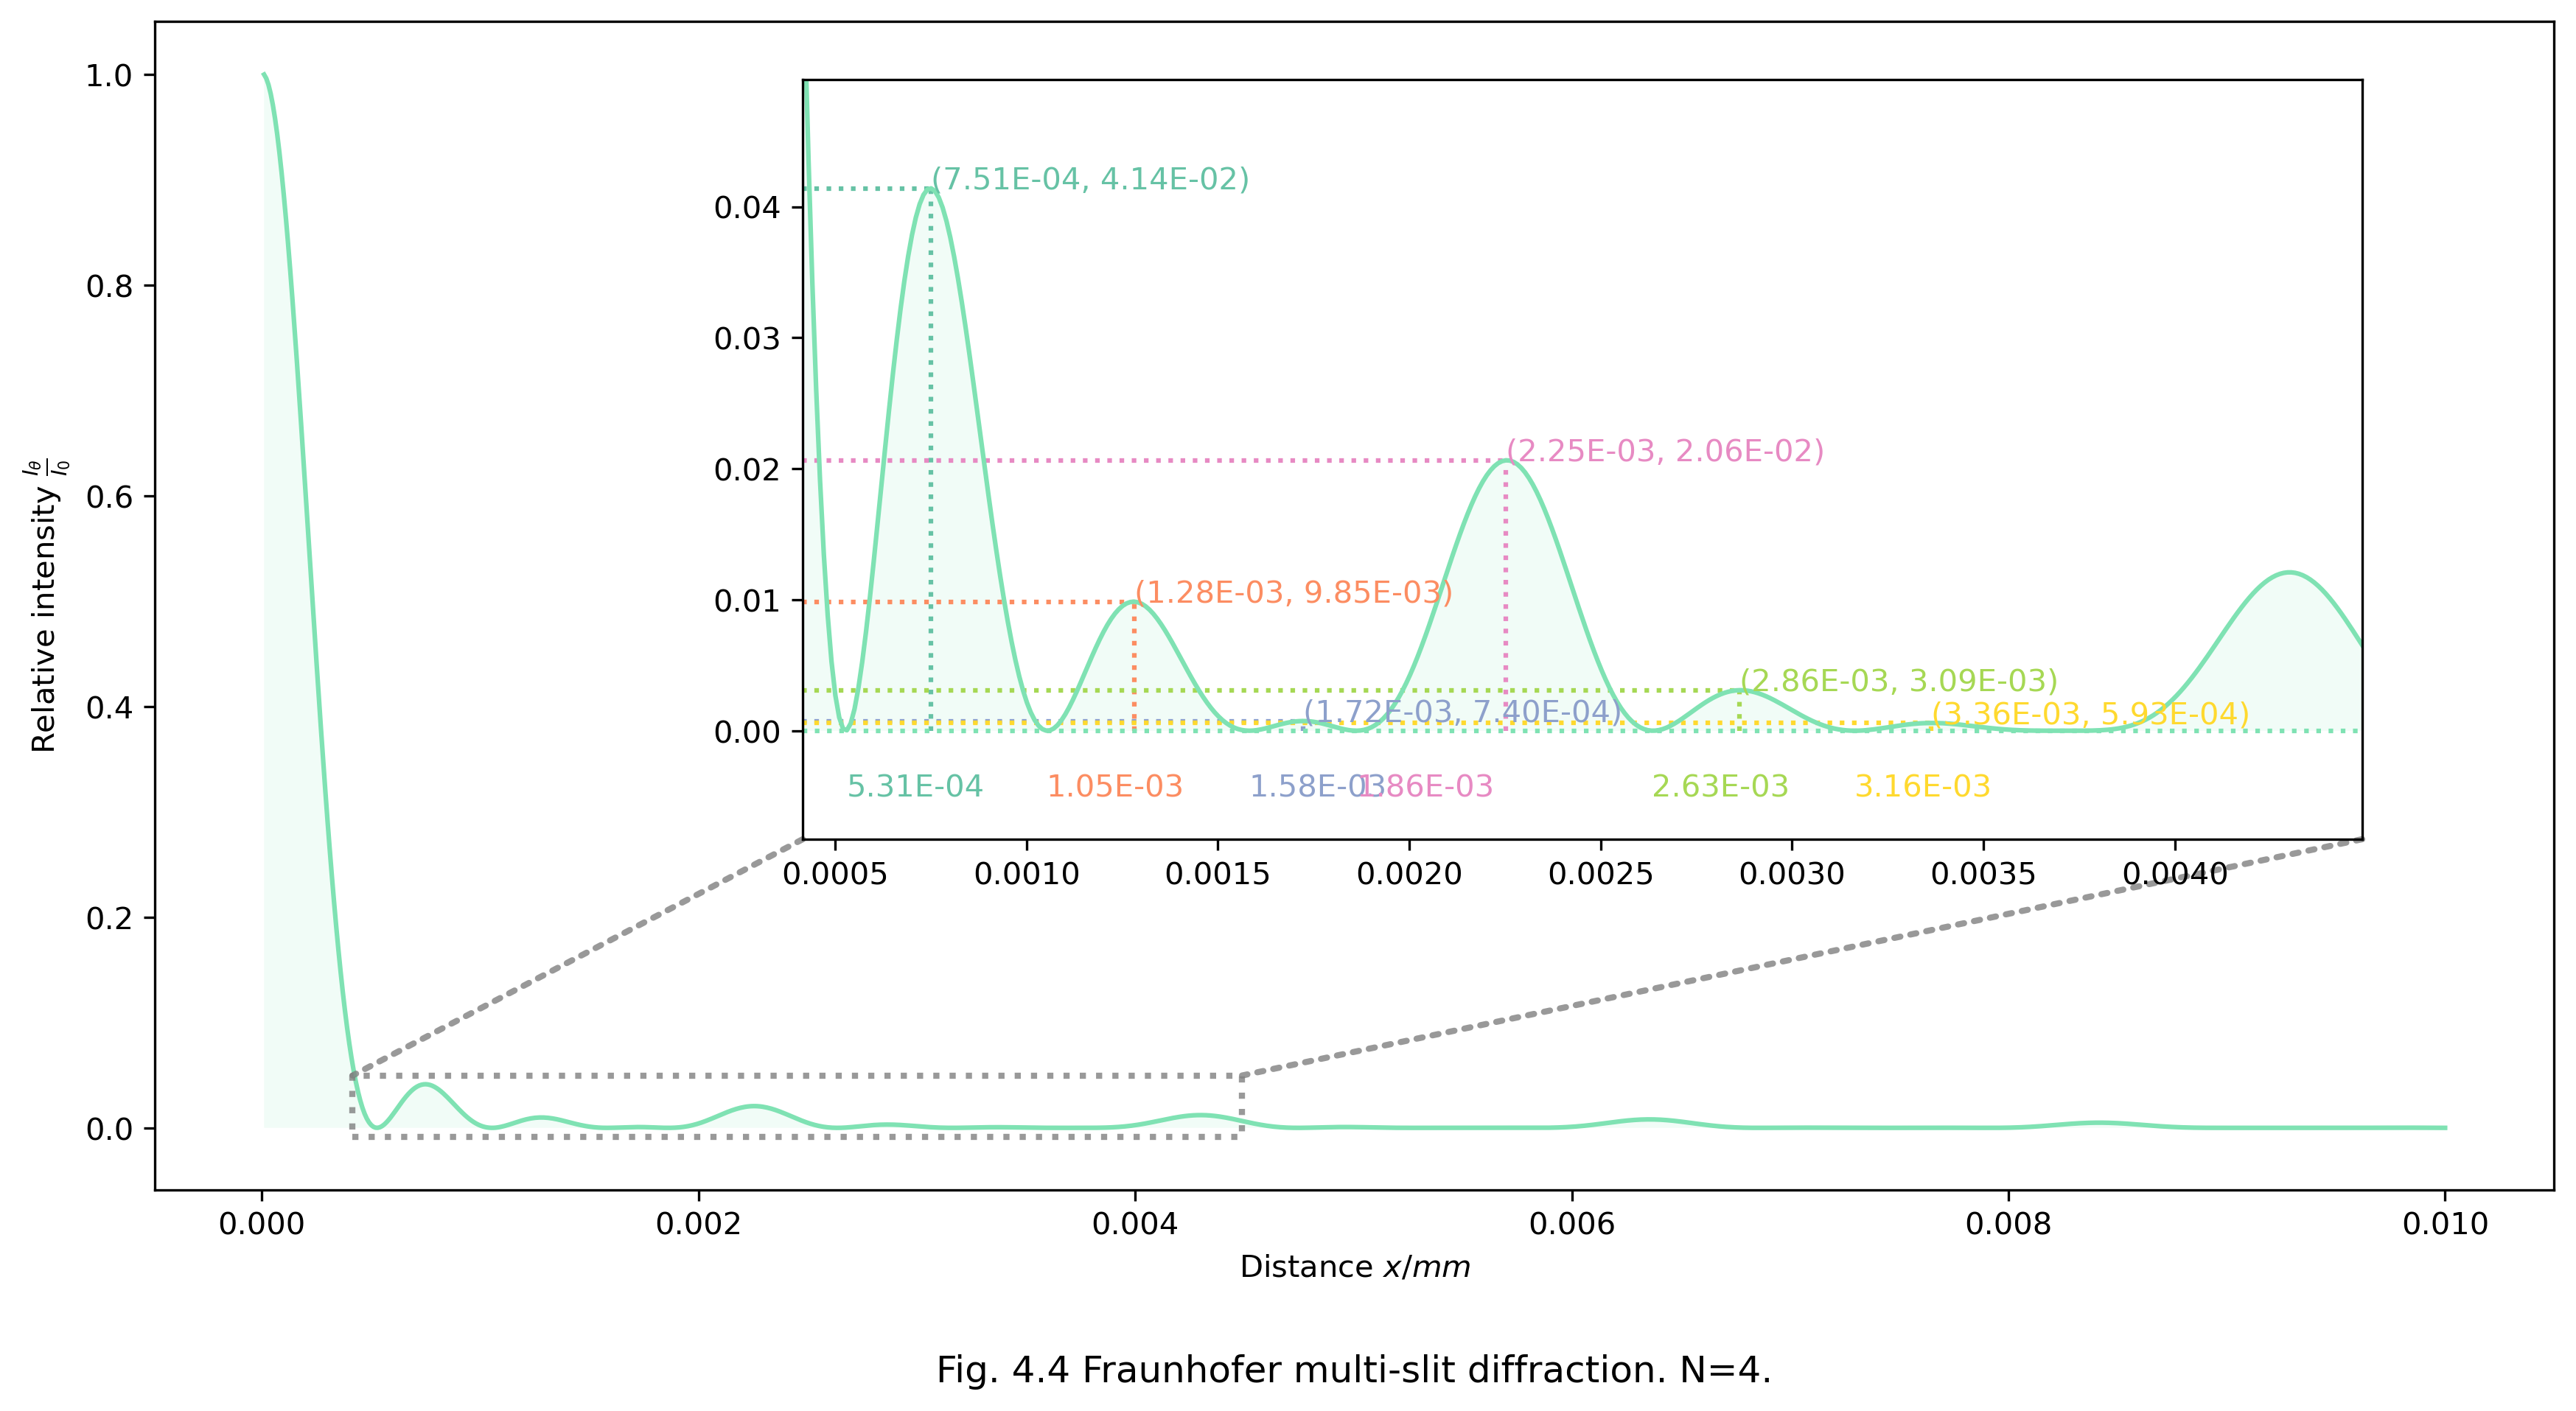
\includegraphics[width=0.5\textwidth]{attachments//Fig.4.4.png}
	}

	\subfloat[N=100]{\label{fig:4.5}
	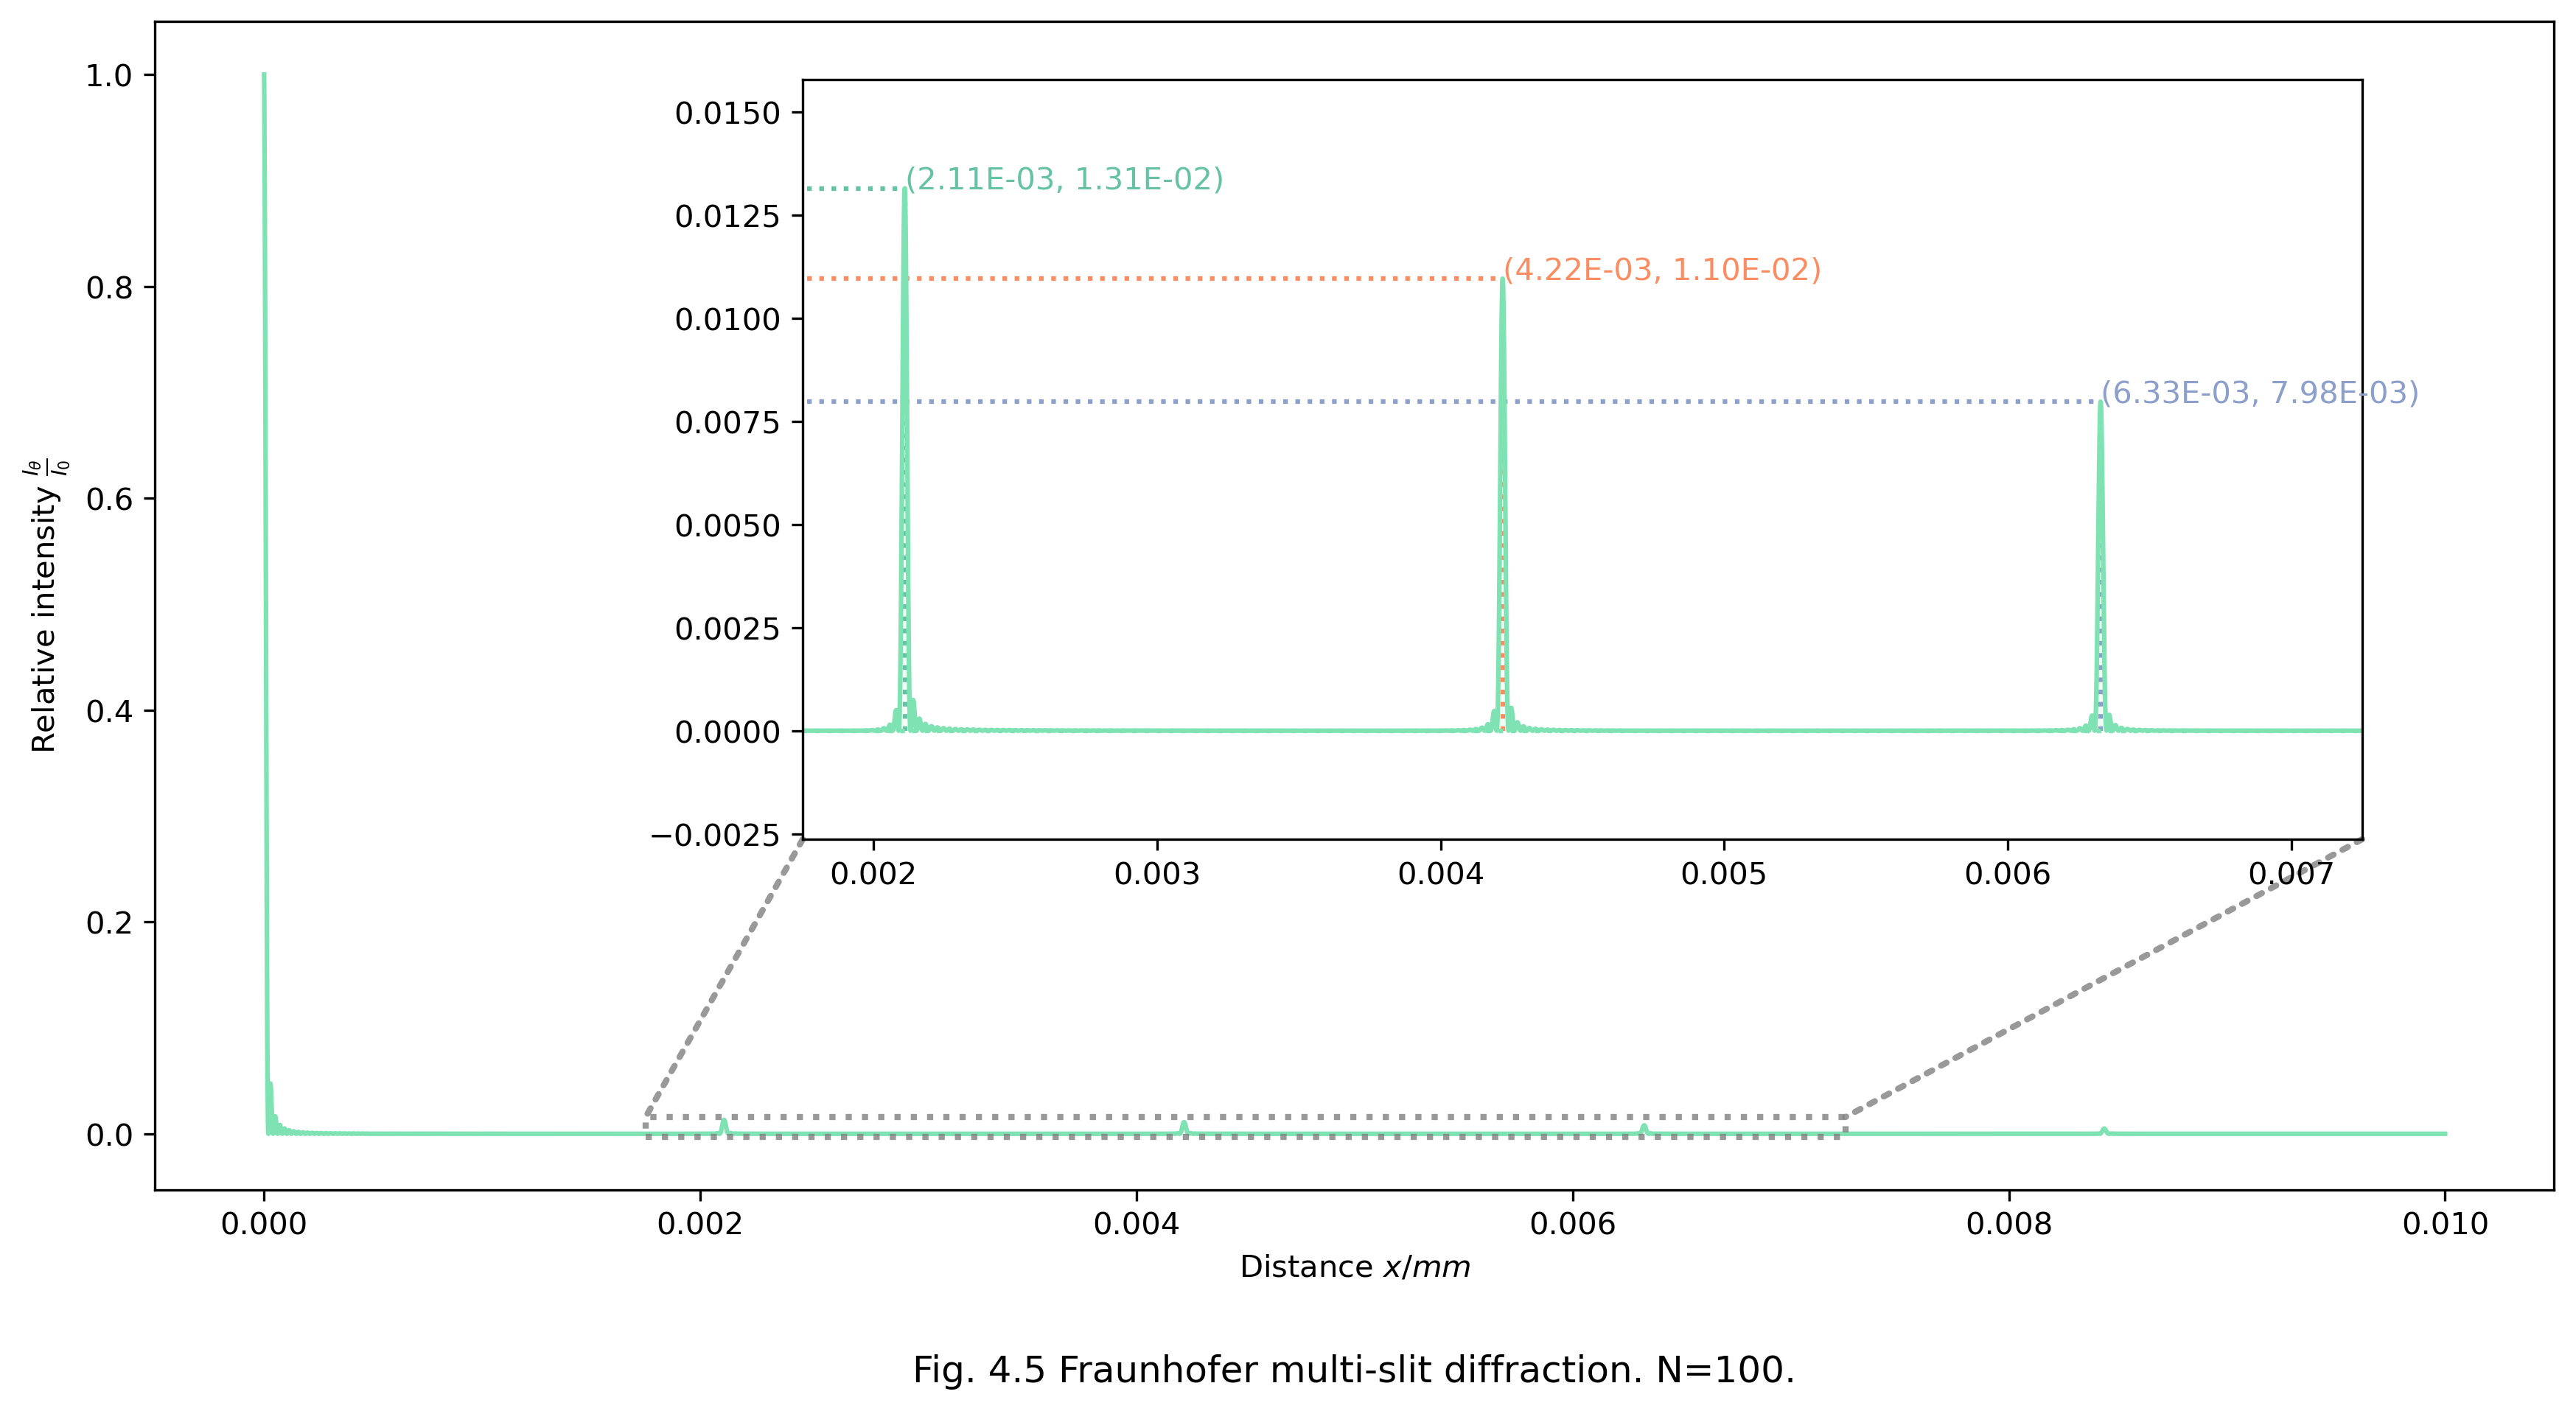
\includegraphics[width=0.5\textwidth]{attachments//Fig.4.5.png}
	}
	\caption{夫琅禾费多缝衍射}
	\label{fig:4}
\end{figure}

\subsection*{【项目源码】}
\href{https://github.com/Jeg-Vet/SYSU-PHY-EXP/tree/main/B10-Fraunhofer_single-slit_diffraction}{SYSU-PHY-EXP/B10 Fraunhofer single-slit diffraction @Jeg-Vet(github.com)}

\end{document}

